%% ----------------------------------------------------------------
%% Thesis.tex -- MAIN FILE (the one that you compile with LaTeX)
%% ---------------------------------------------------------------- 

% Set up the document
\UseRawInputEncoding
\documentclass[a4paper, 12pt, oneside]{uet_thesis}
  % Use the "Thesis" style, based on the ECS Thesis style by Steve Gunn
\graphicspath{{Figures/}}  % Location of the graphics files (set up for graphics to be in PDF format)
%\renewcommand{\chaptername}{}
\usepackage{titlesec}
\usepackage{hyperref}
\titleformat{\chapter}[hang] 
{\normalfont\huge\bfseries}{\thechapter}{1em}{} 
% Include any extra LaTeX packages required
\usepackage[square, numbers, comma, sort&compress]{natbib}  % Use the "Natbib" style for the references in the Bibliography
\renewcommand{\cleardoublepage}{}
\usepackage{verbatim}  % Needed for the "comment" environment to make LaTeX comments

%\usepackage{vector}  % Allows "\bvec{}" and "\buvec{}" for "blackboard" style bold vectors in maths

\usepackage{url}
\usepackage{natbib}


\hypersetup{urlcolor=blue, colorlinks=true}  % Colours hyperlinks in blue, but this can be distracting if there are many links.

% remove the unnecessary spacing before and after the headings/subheadings

\titlespacing{\chapter}{0.1cm}{0.1cm}{0.1cm}
\titlespacing{\section}{0pt}{*1}{*1}
\titlespacing{\subsection}{0pt}{*0}{*0}
\titlespacing{\subsubsection}{0pt}{*0}{*0}

\setlength{\parskip}{6pt}
%\setlength{\parsep}{0pt}
%\setlength{\headsep}{0pt}
%\setlength{\topskip}{0pt}

%% ----------------------------------------------------------------
\begin{document}
\frontmatter	  % Begin Roman style (i, ii, iii, iv...) page numbering

% Set up the Title Page
\title  {An EEG Based System for Advertisement Impact Assessmen}
\session {2016 -- 2020}
\advisor {Dr. Usman Ghani}
\authors {  % please enter the students names and registration numbers
\quad  2016-CS-251\\ \quad 2016-CS-259\\ \quad 2016-CS-262\\ \quad 2016-CS-264 }

\addresses  {\deptname \\ \univname}  % Do not change this here, instead these must be set in the "Thesis.cls" file, please look through it instead
\date       {\today}
\subject    {}
\keywords   {}

\maketitle
%% ----------------------------------------------------------------

\setstretch{1.3}  % It is better to have smaller font and larger line spacing than the other way round

% Define the page headers using the FancyHdr package and set up for one-sided printing
%\fancyhead{}  % Clears all page headers and footers
%\rhead{\thepage}  % Sets the right side header to show the page number
%\lhead{}  % Clears the left side page header

%\pagestyle{fancy}  % Finally, use the "fancy" page style to implement the FancyHdr headers


%% Select only one of the certification pages  
%\CertificationMSc{}
\CertificationBSc{}
\clearpage  % Certification ended, now start a new page


%% ----------------------------------------------------------------
% Declaration Page required for the Thesis, your institution may give you a different text to place here
\Declaration{
%\addtocontents{toc}{\vspace{1em}}  % Add a gap in the Contents, for aesthetics

We declare that the work contained in this report is ours, except where explicitly stated otherwise. In addition this work has not been submitted to obtain another place.

\bigskip

Signed:~~ \rule[0em]{10em}{1.0pt} \\ % This prints a line for the signature 
Date:~~~~ \rule[0em]{10em}{1.0pt}  % This prints a line to write the date
}
\clearpage     % Declaration ended, now start a new page

%% ----------------------------------------------------------------

\setstretch{1.3}  % Reset the line-spacing to 1.3 for body text (if it has changed)

% The Acknowledgements page, for thanking everyone
\acknowledgements{
%\addtocontents{toc}{\vspace{1em}}  % Add a gap in the Contents, for aesthetics

This feasibility report may not be completed without the support and guidance of our supervisor Dr. Usman Ghani who greatly shared his wisdom with patience that helped us in to do research work in an efficient manner.  We also want to appreciate the efforts of our co-advisor Ms. Beenish for giving the suggestions to deal with the technical details of our project. \\
We would like  to give credits to our teacher, parents, colleagues and friends for spending a lot of time and encouraging us to push beyond our limits. Above all, we give our sincerest gratitude to Allah Almighty without Whom nothing would have been possible.


}
\clearpage  % End of the Acknowledgements

%% ----------------------------------------------------------------
% End of the pre-able, contents and lists of things
% Begin the Dedication page
\setstretch{1.3}  % Return the line spacing back to 1.3
\pagestyle{empty}  % Page style needs to be empty for this page
%\dedicatory{For/Dedicated to/To my\ldots}


%% ----------------------------------------------------------------
%\pagestyle{fancy}  %The page style headers have been "empty" all this time, now use the "fancy" headers as defined before to bring them back

%% ----------------------------------------------------------------
%\lhead{\emph{Contents}}  % Set the left side page header to "Contents"
\tableofcontents  % Write out the Table of Contents
\newpage
%% ----------------------------------------------------------------
%\lhead{\emph{List of Figures}}  % Set the left side page header to "List if Figures"
\listoffigures  % Write out the List of Figures
\newpage
%% ----------------------------------------------------------------
%\lhead{\emph{List of Tables}}  % Set the left side page header to "List of Tables"
%\listoftables  % Write out the List of Tables

%% ----------------------------------------------------------------
\setstretch{1.5}  % Set the line spacing to 1.5, this makes the following tables easier to read
\clearpage  % Start a new page
%\lhead{\emph{Abbreviations}}  % Set the left side page header to "Abbreviations"
%\listofsymbols{ll}  % Include a list of Abbreviations (a table of two columns)
{
% \textbf{Acronym} & \textbf{W}hat (it) \textbf{S}tands \textbf{F}or \\
%\textbf{LAH} & \textbf{L}ist \textbf{A}bbreviations \textbf{H}ere \\
}

%% ----------------------------------------------------------------
% The Abstract Page
\addtotoc{Abstract}  % Add the "Abstract" page entry to the Contents
\abstract{
%\addtocontents{toc}{\vspace{1em}}  % Add a gap in the Contents, for aesthetics

Advertising is very important for marketing purposes to maintain their advertising quality. This can be done by knowing the person’s genuine feedback about the advertisement. In this project we will use a low cost EEG headset for collecting the brain signals of the subjects, viewing the advertisements, that aims in providing the statistics of the advertisement's impact and the likelihood of a person purchasing the advertised product. 
By the analysis of brain signals using the latest methods we will be able to distinguish between different brain waves like alpha, beta, gamma and delta each of them being specific to a certain kind of activity.This analysis will help us provide the statistical trend for a certain kind of advertisement on the basis of various factors. 
This will greatly help the marketing sector of multinational companies to improve their advertising campaign which will bring a revolutionary change in how they perceive their brand.

}
\clearpage  % Abstract ended, start a new page

%% ----------------------------------------------------------------
\mainmatter	  % Begin normal, numeric (1,2,3...) page numbering
%\pagestyle{fancy}  % Return the page headers back to the "fancy" style
\onehalfspacing
% Include the chapters of the thesis, as separate files
% Just uncomment the lines as you write the chapters

%% Chapter 1

\chapter{Introduction} % Write in your own chapter title
\label{Chapter1}
\lhead{Chapter 1. \emph{Introduction}} % Write in your own chapter title to set the page header

\section{Introduction}
\subsection{Overview of Project}
Outdoor and indoor localization is an integral component of  IoT (Internet of Things) in this era of mobile computing. Indoor localization can open new horizons for ubiquitous applications targeting university departments, government small institutes, software houses, airports, shopping malls, museums etc. Our project will find the location of a specific person by using appropriate machine learning approach using BLE based Android application. This location will be used to provide guided tour of the indoor building (Computer Science and Engineering Department at UET, Lahore) we will use to validate our work. 

This project will guide persons who are not much familiar with visiting place. It has an android application that will predict the indoor location of a person at room level and also gives information of current room location and nearby rooms in the form of text, images, audio and videos. In our case visiting place will be CSE dept at UET LHR. For room prediction, RSSI fingerprints of BLE beacons will be captured for training of model. After finding the location of the person, guidelines of that certain room/area will be provided to the user on user end Android application. Indoor positioning has numerous applications. We can use indoor positioning of people to guide them inside shopping malls, airports or museums. 


Indoor positioning systems can be broadly classified into two main parts: Systems that need some infrastructure which are further categorized into those which needs ad-hoc deployment  like BLE beacons and systems which takes profit of previously installed infrastructure like WiFi fingerprinting technique. Those technologies which do not need any infrastructure deployment are based on magnetic field fingerprinting. Ad-hoc deployment can be initiate in new areas where there is need to save environment from magnetic rays or in those areas where WAPs are weak so we choose to detect indoor location using BLE beacons.Also,  BLE based indoor  localization is wireless, consumes low power because it works on battery and mostly available in smart mobile devices.

BLE can be used from two different approaches: trilateration and fingerprinting. In tilateration relationship between the user's RSSI measurement and its distance to the BLE beacon station is considered. By estimating distances to multiple beacon stations, the user's location can be predicted using a least square algorithm. The  fingerprinting approach is implemented in two phases: an ofliine phase and an online phase. The ofline phase is called the training phase. During this phase, fingerprint  RSSI values are determined of every beacon from each device location. The online phase is known as the localization phase which is the actual prediction of the user's device location.

\textbf{What are BLE beacons?}

Beacons are small, wireless transmitters that use low-energy Bluetooth technology to send signals to other smart devices nearby.They are probably the most recent advancement in area innovation and closeness advertising. Set forth plainly, they associate and transmit data to savvy devices making area based prediction and are progressively precise.Each tool contains a CPU, radio, and batteries, and it really works by means of again and again broadcasting out an identifier. This identifier is picked up by way of your tool, commonly a cellular, and marks out an crucial area for your surroundings. The identifier is a unique ID variety that your phone recognizes as specific to the beacon. Once related, the beacon will carry out the signals for what we are using it. 
\begin{figure}[h]]
\begin{center}
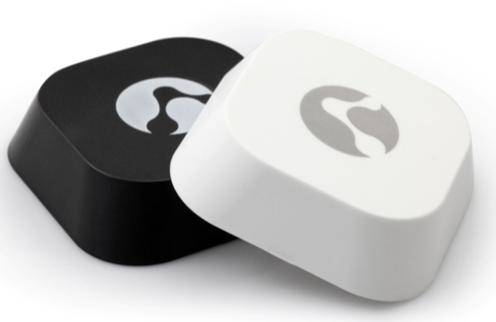
\includegraphics[scale=0.6]{beacon}
\caption{Beacons}
\label{fig:1}
\end{center}
\end{figure}


\textbf{Why we are using BLE beacons?}

In this evergoing techinal era, everyone wants leisure and his needs in less time and cost. He wants to become smart.So, due to mentioned reasons we are using this technology.
\begin{itemize}
\item Beacons are small, wireless sensors that are normally placed in a casing, have low power consumption because they work on battery.
\item The technology uses Bluetooth Low Energy (also called Bluetooth Smart or Bluetooth Version 4.0+) to broadcast radio signals or, simply put, to communicate with other smart devices.
\item The broadcasted beacon signals can be captured by smart gadgets, like phones, to call ad-hoc actions.
\item Under the beacon’s casing, there is a small ARM computer with a Bluetooth Smart connectivity module, which is powered by a battery.
\item The module runs on firmware, a piece of software installed on beacons.
\item As the computing power is limited, it can be used for processing sensor data (information about signal power) and encrypting a beacon’s ID. There is a small antenna from the CPU.
\item The antenna is built in to broadcast electromagnetic waves with specific length and frequency (2.4 GHz radio waves).
\item This technology is primarily used for mapping and location services using the RSSI (received signal strength indicator) estimate. 
\end{itemize}

\subsection{Background}
Outdoor localization has been formalized by using satellite-based technologies i.e. GPS\cite{GPS}, BeiDou\cite{cooper2016loco}, GLONASS\cite{cooper2016loco}, and GALILEO\cite{GALILEO}. It is hard for finding the indoor location by using conventional GPS technology because of no direct (Line of Sight)\cite{akram2018censloc} in indoors, so we cannot use these technologies for indoor positioning. Up to date, the technologies used for indoor localization approach are: TOA (Time of Arrival), TDOA (Time Difference of Arrival), AOA (angle of arrival) but they have some limitations. TOA and TDOA require precise clock count and its synchronization and AOA-based systems require special antennas for their propagation. 
By keeping in view the evergreen trend of engaging users towards something is through mobile computing.So, there exists some systems which used magnetic rays, time of arival of specific signals, some used WiFi based localization and also deployed on Apple and Android smart phones but due to coherence and interference of different signals in determining the RSSI of fixed WAPs, crucial errors occurred. By analyzing these calculations, we are able to avoid multiiteration(which predict location of device by determining the distance between the AP and mobile device) and capture fingerprints from multiple mobile devices.

The indoor positioning system which we are using is communicating with hardware device so we require a technique which translates the signal into a location. There are three categories to transform this: proximity, geometric and scene analysis,. Proximity methods create zones and assigns the users location when they enter that zone. Geometric method uses signal measurements from device locations and put them in geometrical equations to predict the location but scene analysis method measures the signal from different refence points by standing at one location and then predicts location by passing that fingerprint to trained model which is called fingerprinting technique. A fingerprint is
a collection of signals received at a certain location in the scene, in this way they aim to make the fingerprint
location specific, such fingerprints are often based on the RSSI values collected from beacons.

So, we are going to implement a system which employs suitable machine learning approach to find the location by using RSSI (Received Signal Strength Indicator) fingerprinting technique because there is less hinderance of other signals in using this technique.. This RSSI values will pass to the trained model (a model which is trained on a given set of input and output values by using appropriate machine learning algorithm) which gives the location of the user's mobile device.



\section{Motivation} 
People/visitors who go to an unknown place find it difficult to traverse and wants to find places/people of interest easily. Such problems motivate us to provide ease and leverage facility to users so that they can see the information of a particular indoor environment on his mobile application automatically. BLE is available on nearly every smart device so no additional hardware required at user end. Hence by utilizing their indoor location determined using machine learning on BLE fingerprints, guided tours of smart campus to visitors can be provided and facilitating them. We are using latest technology of BLE beacons because they work on battery and consume less energy than Wi-Fi signals\cite{hultgren2015evaluating}.

\section{Objectives of the project}
\subsection{Industry Objectives}
\begin{itemize}
\item Implement a system that takes into account the demands of university campus exploration.
\item This project leads to visitors of any organization or store to save their time and effort by providing them textual and pictorial information of organization or store.
\item Administrators seek advantage of their time by providing much information to their customers in less time which automatically increase the sales and profit of their product.

\end{itemize}
\subsection{Research Objectives}
\begin{itemize}
\item To find the location of the user that will be connected to his Android app via Bluetooth technology\cite{Introduction}.
\item To monitor and provide guidelines to user who is connected to the BLE beacon via Bluetooth and mobile application, we need to find user location inside buildings.
\item To understand the concept of Android application development which provide textual and pictorial information of particular area and its nearby areas to the user who is located in that indoor environment.


\end{itemize}
\subsection{Academic Objectives}
\begin{itemize}
\item This project enables us to understand the concepts of following subjects:
\\a.	Machine learning
\\b.	Networking
\\c.	Android development
\\d.	Front-end design
\\e.	Client server communication management
\item To complete a whole real world project , utilizing concepts from computer networking, databases, machine learning, software development life cycle of SE , testing and mobile development.
\item To develop the understanding and connection between the Android app and the hardware structure. 
\item To find the best Machine Learning algorithms which are used to train the model of fingerprints. 
\item To make an Android application which use as an interface to provide guidelines to the user who is located in a particular indoor environment.
\item To ensure the use of latest technologies in implementing the project which helps technical persons and students to enhance their academic skills via learning new features


\end{itemize}

\section{Scope of the project}
In this project, android application runs on a user’s mobile device and and will capture BLE RSSI fingerprints. The fingerprints collected at the initial stage will be processed and used to train suitable machine learning model, after training of the ML based location prediction model, based on the room prediction relevant information of nearby rooms, facilities and personnel available will be prepared to be displayed to user at run time , the user will be guided to install our Android app on their phone, their mobile device will capture BLE fingerprint and the fingerprint will be sent to back end server where our trained model will predict their current location inside building in terms of room\cite{Loco}. The relevant information will be delivered and shown on user mobile device providing guided tour. 
The placement of Bluetooth low energy beacons will be held in CSE dept at UET Lahore. 


\section{Target Audience}
Targeted audience will be the:
\begin{itemize}
\item Visitors of the University campus 
\item New Students and Staff of the campus
\end{itemize}



\section{Possible Applications of work}
The possible application of work for our project are as follows:


\begin{itemize}
\item Software house information (Development, QA, Frontier)
\item Airport assisting system
\item University Campus smart information system
\item Government small Institutes
\item Medical departments exploration in hospitals
\end{itemize}


\begin{table}[h]
\centering
\begin{tabular}{l|l} \hline
\end{tabular}
%\caption{Flow in the logic}
\label{tab:logic_flow}
\end{table}




 % Introduction 
%
%% Chapter 2

\chapter{Literature Review and Problem Statement} % Write in your own chapter title
\label{Chapter2}
\lhead{Chapter 2. \emph{Literature Review and Problem Statement}} % Write in your own chapter title to set the page header

\section {Description and scope of the related literature}
This study aimed to focus on detailed analysis of existing literature related to our project that includes literature review of indoor and outdoor localization techniques, their performance, their contributions and their shortcomings. 

In recent times, indoor localization can open new horizons for fascinating and useful applications targeting university campuses, government institutes, airports, shopping malls, museums etc. We can provide different kinds of information by using indoor location of the person. This will be extremely beneficial not only in university campus but also in airports and shopping malls. Shopping malls can use this kind of application by providing much information to their customers in less time which automatically increase the sales and profit of their product. But our purpose is that to provide the ease to the users who visit our department. Our project can be extensible to other areas where it can provide huge benefits to the businesses. But we are specifically focused on providing guidance to the visitors of our department. In this way our project will be used as a guidance tool. 

Our project is innovative in the sense that we use indoor location of a person by providing him/her smart guided tour of our department but mostly existing systems uses indoor location of a person for different purposes like providing assistance to older age people. We are not interested in their purposes, but we have great interest in existing indoor localization techniques. So the scope of this literature review will cover all well-known existing indoor localization techniques. But before going on detailed study of indoor localization, we have to study about outdoor localization in order to find how they work and why we can’t use outdoor localization technique in indoor environment and then we delve into indoor localization techniques. 


\section {General findings and availability of the literature}

As I stated, that mostly existing systems uses indoor location of a person for different purposes like providing assistance to older age people. But there exist a research\cite{AR} that presents a mobile campus tour application based on augmented reality in various universities and the features of application are the information about points of interest, location search and navigation, but it provides outdoor locations of large university campus using GPS, because it is not based on room level prediction and information about indoor locations. But the huge literature related to indoor localization presented various indoor techniques and analysis of their performance measures is available on internet in which we are interested.  

\section{GPS Outdoor Technology}
GPS (which is known as Global Positioning System) is the satellite navigation system. It is used for outdoor localization. It tells us where you are on the earth. It retrieves information of time and position where you are on the earth in all weathers. GPS was developed by United States military in 1960 and it is used in next few decades.First of all, it is used for civilian purpose. Today, we use GPS in many technological devices such as GIS device, mobile phones and many watches. The area of application of GPS includes land, space, air and marine. The GPS system is made up of 5 ground stations and 24 satellites where each satellite placed in precise orbit at an altitude of 10,900 miles \cite{GPSworks}. As we all know, we used GPS as outdoor locating services. It receives signals from at least three satellites and uses triangulation and trilateration technique which is used to calculate the position of the object. It calculates the distance of a receiver from each satellite where distance is calculated by time it takes for a radio wave to reach the receiver end. GPS can be used in any type of weather and it also provides timing information. Here is the illustration of how GPS works.
\begin{figure}[h]
  		\centering
    		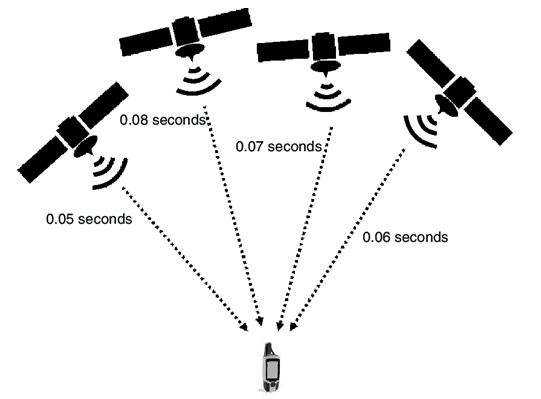
\includegraphics[scale=0.6]{./Figures/GPS}
 		\end{figure}
    
GPS does not work in indoor location because of no direct line of sight in indoor area. Here are some limitations:
\begin{itemize}
\item GPS signals carry waves at a frequency that is scattered by solid objects usually by buildings and walls.
\item Actually, satellites sent the signals that are not easily penetrate all kinds of barriers.
\item	When signal enters into the building, then it gets distorted due to construction material such as wood, bricks, cements etc because it serve as hindrance to the satellite signal.\cite{IP}

Hence, we can’t use outdoor localization technology like GPS in indoor environment.
\end{itemize}


\section{Indoor Localization Techniques}
Indoor localization techniques become popular day by day because it can provide ubiquitous location based services to people. Indoor positioning systems consist of a network of transmitters used for locating persons inside buildings. Here are the popular approaches: 
\subsection{Triangulation}
Triangulation technique uses the geometric properties of triangles in order to find the position of the object. In triangulation, AOA (Angle of Arrival)\cite{Sakpere2017ASS} technique is used to measure the angle and distance relative to two or multiple fixed points through the intersection of direction lines between the fixed points and then this information is used to calculate the position of transmitters which in turn describes the actual location of object.  In other words, position of target object is determined by the intersection of direction lines. Here is the illustration of this technique.
\begin{figure}[h]
  		\centering
    		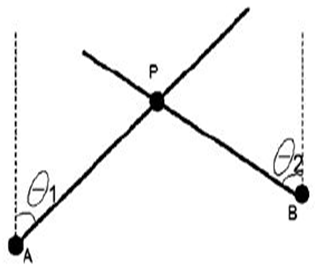
\includegraphics[scale=0.7]{./Figures/triangulation}
 		\end{figure}

\textbf{Drawbacks of Triangulation}

This method achieves good results outdoors but it gives weak results inside the building because the radio signals emitted by transmitters get attenuated by several obstacles hence it gives poor estimation of distance calculated. Moreover hardware requires special antennas for signal propagation and hardware requirement for the coverage of large area tends to be expensive and complex\cite{Sakpere2017ASS}. When the area becomes large with multiple reference points, accuracy will decreases due to some errors in the estimation of distance calculated.

\subsection{Trilateration}
Trilateration is also used to estimate the position of object using geometric properties of triangles. The position of target object is determined by TOA (Time of Arrival) and TDOA (Time difference of arrival) \cite{Sakpere2017ASS}. TOA is used to estimate the position of target object by calculating the time taken by a signal to reach the receiver from transmitter. TDOA is the improved version of TOA that considers the difference in TOA at two different receivers and then finds the relative position of transmitter based on the difference which further used to estimate the location of target object. This results in higher accuracy.

\textbf{Drawbacks of Trilateration}

The cost and complexity of hardware is high and it does not give good enough estimates in indoor area because of the inherent error of the distance measure calculations, hence most results have several meters of error\cite{cooper2016loco}. The accuracy is also affected by environmental conditions. In order to get good results both transmitter and receiver require precise clocks that should be synchronized. 

\subsection{Proximity}
Proximity technique is also used to estimate the location of target object. It requires a grid of antennas with known locations. When mobile device is detected by more than one antenna, then the antenna with the strongest signal is used to calculate its position. The position of target object (mobile device) is determined by using RSSI (Received Signal Strength Indication) to estimate the distance between mobile devices in order to get the position information of device.

\textbf{Drawbacks of Proximity}

Although proximity is applied on the systems using Bluetooth, IR but it requires calibration effort\cite{Sakpere2017ASS}. Also, we need larger spread of readers in order to achieve a reliable system but it increases system complexity and cost.

\subsection{Fingerprinting technique (Our Selected Approach)}
Fingerprinting technique is based on pattern matching technique. It is used to create signal strengths database that are based on the RSSI (Received Signal Strength Indication) values of various APs. These values are collected at different locations of an experimental area. These are called fingerprints, then by applying any machine learning approach we can train the model which further uses to predict the location of target user. Fingerprinting technique has a better positioning performance and accuracy as compared to the others and it doesn’t require any software or hardware modifications at transmitters end.

Here are the \textbf{indoor positioning technologies} which uses mostly any of method described above to predict location:

\textbf{1. Infrared (IR) positioning systems}

This system consists of a network of IR sensors that are linked by wires and then connected to a centralized server. Early badge system uses IR sensors for determining the position of object or people who is wearing badge.  Active Badge system uses IR sensors and TOA approach for estimating the location. Theses sensors are cheap and have good battery life. But the problem is that people have to wear the badge. This problem is solved by using IR thermal sensors\cite{Sakpere2017ASS} that uses the thermal rays emitted from human body for the prediction of location. Because we know that the temperature of human body is differs from room temperature.

\textbf{Drawbacks of IR positioning systems}

We need larger number of IR sensors to cover the large area which in turn increases system complexity and cost. Also these systems have limited accuracy. Thermal IR sensors also have major drawback that human body is not only the source of heat, there are also other heat sources like electronic devices and light bulbs that could affect the signals received from thermal IR sensors.

\textbf{2. Ultrasonic positioning systems}

This system contains ultrasonic sensors that emit ultrasonic signals which are used to estimate the location of object by measuring the TOF (Time of Flight) \cite{UPS}. The distance between transmitters and receiver is calculated by TOF and then this information is used to estimate the target position.

\textbf{Drawbacks of ultrasonic positioning systems}
This system is expensive and difficult to implement and maintain on larger area. Also, the ultrasound signals have low signal propagation speed when compared to speed of light\cite{Sakpere2017ASS}. It also affects by hindrances in indoor environment which in turn reduces its accuracy.

\textbf{3. Image based indoor localization}

It is a visual-based localization method. Early visual based methods require feature detection and matching that require huge computation and also it is affected by environmental conditions. There is a literature that implements this system by different approach. According to this research, firstly we need to build a database that contains collected images of experimental area. CNN (Convolution Neural Network) is used to train the model which is further used to predict the location of target object by inputting it the image of target location.\cite{image}

\textbf{Drawbacks of image based indoor localization}

Clearly, use of camera might be obtrusive for some users. Also time consuming effort is required to build the dataset and it also has scalability issue. Also, if we take image from different point of view which is not present in database, it might be possible that it would be predicted wrongly which in turn results the low accuracy. 

\textbf{4. Zigbee and capacitive sensors}

Zigbee sensors \cite{AAL} are also used for indoor location but they are very expensive and have medium scalability. Capacitive sensors \cite{AAL} are also used to estimate location by pressure sensing that detects the presence of a person but this system is very impractical to implement and deployment of sensors in floor is expensive.

\textbf{5. Wi-Fi based indoor localization}

In this, we can use either triangulation technique or fingerprinting technique for the estimation of the location of target user. But in triangulation, we require modification and special software to run on Wi-Fi base stations \cite{AAL}. But fingerprinting technique with Wi-Fi is a good approach for indoor localization because, we didn’t need any additional hardware for this system and we can use already deployed infrastructure. 

\textbf{Drawbacks of Wi-Fi based indoor localization}

Its main drawback is that it consumes more power. There are some spots where Wi-Fi access points would be difficult to power. There are some areas where Wi-Fi signals are not accessible. \cite{cooper2016loco}

\textbf{6. BLE beacons based indoor localization (our approach)}

After seeing the drawbacks of existing technologies, we decided to find the indoor location of a person using BLE beacons with fingerprinting technique, because it overcomes many drawbacks in existing systems, also they give better accuracy.  BLE beacons are Bluetooth low energy beacons. Classic Bluetooth consumes more power than BLE beacons and transmits to long ranges. BLE beacons are small in size, light weight and cheaper then Wi-Fi. BLE consumes less power than Wi-Fi. BLE beacons are usually battery powered, which are more flexible and easier deployed than sensors used by existing systems. BLE signals have higher sample rate than Wi-Fi signals. BLE consumes much less power because it transmits data over the small range \cite{BLEguide}. Bluetooth having version greater than 4.0 are BLE. BLE Beacon is a tiny device with a massively used for broadcasting of signals. It has unique ID (MAC Address). A BLE beacon has three major components:  ARM computer, a Bluetooth connectivity module and batteries for powering the entire circuit. The antenna is attached to the CPU of ARM computer. It broadcasts electromagnetic waves with specific length and frequency. Here is the internal circuitry of BLE beacon.

\begin{figure}[h]
  		\centering
    		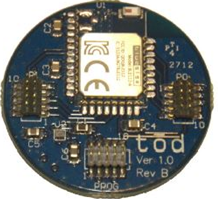
\includegraphics{./Figures/internalbeacon}
 		\end{figure}

Android phones with 4.3 and 4.3+ version support BLE \cite{BLEguide}, which makes it easy to implement. 
\\
\textbf{Conclusion}

As we can see there are many drawbacks in existing systems. In some systems, camera is required for indoor positioning which is obtrusive for some users. High cost and effort is required for the deployment of indoor localization infrastructure. Triangulation and trilateration proximity techniques require modifications at hardware end (Wi-Fi work stations) for the purpose of these techniques to work. These techniques also didn’t give satisfactory results in indoor environment due to the errors in distance measure calculations. Proximity technique also requires calibration effort and it is a costly technique to implement. Fingerprinting technique seems to be most suitable that’s why in our proposed system we use this technique. Most of the other existing systems have medium or low accuracy. In image based indoor localization, time consuming effort is required to build data sets. Wi-Fi fingerprinting is relatively better than other systems because of finding position by using already deployed infrastructure. But its main drawback is that it consumes more power. There are some spots where Wi-Fi access points would be difficult to power. So, after analyzing the drawbacks of existing technologies, we find out that BLE beacons with fingerprinting approach is most suitable because of various reasons that I have described above.

\section{Applications of GPS}
There are many applications of GPS which are as follows:
\begin{itemize}
\item Machinery and Information Technology for Bio Mass Production
\item Mobile Robot Sensors
\item Traffic sensing Technologies
\item Sensors and computing systems in Smart Clothing
\item Radio Navigation Systems
\end{itemize}
\textbf{Why we can’t use outdoor localization technology in indoor environment?}




\section{Problem Statement}
Whenever a visitor goes to university campus or visits a new place, he does not know about the specifications of that area i.e. what happens in that specific room or what courses have been taught in a particular and its nearby labs. So, we are developing a system which assists them in determining the textual and pictorial information of a particular area and its nearby locations. For this purpose, we first find the indoor location of a user by using BLE beacons and RSSI values, and then provide information to him automatically on his Android application.  % What to Write 

%% Chapter 3

\chapter{Dataset} % Write in your own chapter title
\label{Chapter3}
\lhead{Chapter 3. \emph{Dataset}} % Write in your own chapter title to set the page header

\section {Dataset Description}
To determine the indoor location of the user, we need a trained model on specific dataset  through which we can predict his location. In order to train our model, we gathered dataset which contains the fingerprints of BLE beacons in Computer Engineering Department. Each beacon has its own MAC address which is used for its identificati n. We have total 24 beacons, that’s why we have 24 input features and each feature contains the RSSI values of specific beacon associated with that feature, and the output is the labeled name of the location. We have total 23 labels which mean we have total 23 classes hence it is a multiclassification problem. RSSI values ranges from -95dBm (low RSSI ~ far off Access point) to - 50dBm (demonstrating high RSSI close to Access point).
\begin{figure}[h]
  		\centering
    		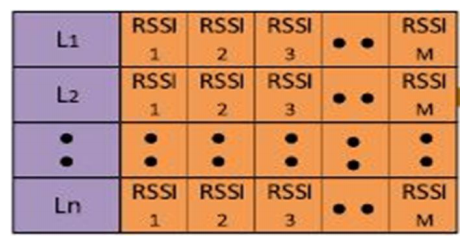
\includegraphics{./Figures/1}
\caption{Dataset format with each label and its corresponding RSSI value}
\label{fig:1}
 		\end{figure}
    

\section {Experimental Area Description}
The experimental area that we covered is the Computer Engineering building of UET, LHR. We skip some rooms of that building because they are locked most of the time. The representation of the deployment of beacons in dept is shown in the following figures. Figure 2 represents the ground floor and Figure 3 represents 1st floor of the building. Small blue circle represent BLE beacon. Following figures only represents those rooms that we have considered in our experimental area. Each room is assigned a label as shown in the figures. Corridors are divided into 4 portions. Each portion is represented by a dotted box and assigned a label shown in the figures. 
\begin{figure}[h]
  		\centering
    		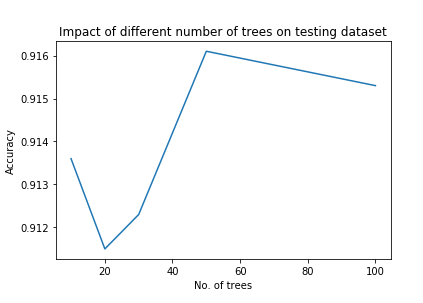
\includegraphics{./Figures/2}
\caption{Map of ground floor of the building where beacons are installed}
\label{fig:2}
 		\end{figure}
    \begin{figure}[h]
  		\centering
    		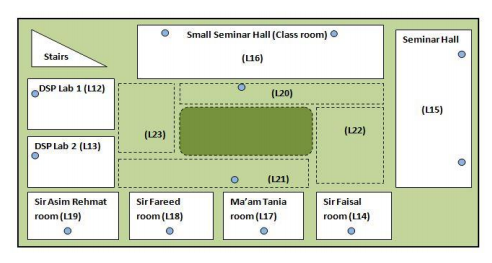
\includegraphics{./Figures/3}
\caption{Map of first floor of the building where beacons are installed}
\label{fig:3}
 		\end{figure}
 \section {Collected Dataset}
Our collected dataset contains 6500 samples of 18 locations of selected area out of 23 locations. Each  location has its own fingerprint RSSI value with respect to certain beacon which depends on different environmental conditions such as distance of device location from the beacon or signal capturing strength of the device. So, we collect samples to predict different locations. The number of samples collected per location is shown in the following figure.
 \begin{figure}[h]
  		\centering
    		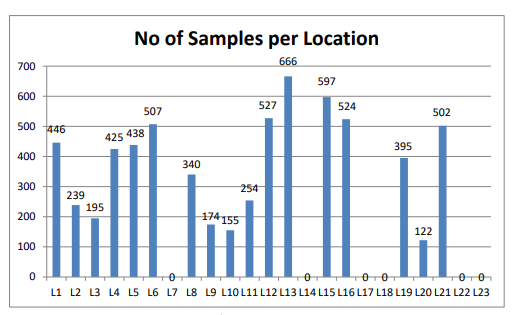
\includegraphics{./Figures/4}
\caption{Number of samples collected for each label}
\label{fig:4}
 		\end{figure}
\\\\
\subsection{Preparation of data set}
When we captured the data, numerous .csv files generated in which each .csv file contain one sample. We used 5 different cell phones for data capturing. Then we compile all the generated .csv files into single .csv file in specific format that we have shown in Figure 1. We discard all those RSSI values of surrounding BLE enable devices which are not from our BLE beacons.
\subsection{Preprocessing of data}
We have done pre-processing on our collected data set. In pre-processing, we have dropped all those rows that have null values in all of their input columns. During data collection some access points are visible, some not hence there were lot of missing values in data set. So, we replace missing values with -100dbm. The reason for replacing the missing values with -100dbm is because it shows extremely weak signal means it is far off from access point. We have not done normalization on our data set because we didn’t find it suitable for our collected dataset.


\subsection{Performance Measures criterion for the comparison of algorithms}
{\bf Accuracy} is the measurement of model performance. It is calculated as the no of samples correctly classified/ total no of samples.
 
\begin{figure}[h]
  		\centering
    		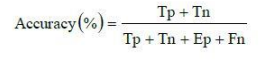
\includegraphics{./Figures/accuracy}
\caption{Accuracy}
\label{fig:5}
 		\end{figure}

{\bf Precision} tells about how accurate your model is out of those predicted positive, how many of them are true positive. Precision is a good measure to determine, when the costs of False Positive is high.

\begin{figure}[h]
  		\centering
    		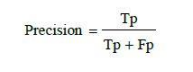
\includegraphics{./Figures/precision}
\caption{Precision}
\label{fig:6}
 		\end{figure}
 
{\bf Recall} actually calculates how many of the Actual Poitives our model captures through labeling it as Positive (True Positive).

\begin{figure}[h]
  		\centering
    		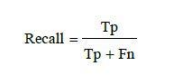
\includegraphics{./Figures/recall}
\caption{Recall}
\label{fig:7}
 		\end{figure}

For calculation of precision and recall for multi-classification, we can calculate the precision and recall separately for each class.
% For example, for class X, we can calculate its precision like that TP_X/Total Predicted X and recall for X class is calculated as TP_X/Total Actually Labeled X.
Then we calculate the average precision and recall of all classes and hence we will get the approximate calculation of precision and recall for them.  % Experimental Setup

%% Chapter 2

\chapter{Research Methodology} % Write in your own chapter title
\label{Chapter 4}
\lhead{Chapter 4. \emph{Research Methodology }} % Write in your own chapter title to set the page header

\section{Introduction}
After the literature review, we conclude that the most of the applications are based on outdoor localization such as GPS. This application only tells the outdoor locations on the maps. When we are out of the building, it’s only shows the boundaries of the buildings not the rooms. But we want to create an application which tells about the indoor location. This application is based on room level prediction. It’s not only tells the room level prediction but also tells the entire information of the room. 
\\
The purpose of writing this chapter is to explain the methodology for making this indoor localization based application. We want to tell that which methods and approaches we used to develop this application. We will also explain that which ML (Machine Learning) algorithms are used, how to collect the data, how to analyze data for this application. We also describe the use cases, use case diagram and test cases of this application. 

\section{Research Methodology}
From the literature review, we conclude that the concept of outdoor localization is introduced on the behalf of GPS. People can access anywhere when he is on the GPS which is installed on every smart phone. But people can only see the boundaries of the building not the rooms of the buildings. They did not know the entire information of the building. They do not know the concept of indoor localization. People face the problem to know the entire information of the building. For example, when a student enters the University for Admission, he/she did not know the ways of the university. They have to face the problem where is Admin block? Where is library? Where is department? Furthermore, if people enter to the hospital, offices, buildings etc., than they did not know the indoor location of those places.  To answer all of these questions, we want to develop the application which tells the indoor location of the building. It not only tells the room name but also tells the entire information of the room. If we talk about the building of the university, then it also tells us the room member name, its office hours etc. We provide this information in the form of texture, audios and pictures.
\\\\
\section{Proposed Work to develop the Android Application}
Actually, we cannot refuse that many indoor applications also developed but they all used different technologies. Most of the indoor applications used Wi-Fi for predict the position of the person that tells the indoor location of that person. But we have to develop the system which tells the indoor location of the person which is based on BLE beacons. BLE beacon is the Bluetooth device which consumes less energy. It is light weight and cheaper than Wi-Fi signals. BLE beacons are usually battery powered, which are more flexible. It is easier to sense the signals. 
We don’t have enough resources to make this application globally. Now, we make this application for our computer Engineering department, UET. To develop this system, we consider the number of points which tells the methods to develop the system that is as follows:
\begin{itemize}
\item First of all, we deploy the BLE beacons in our department. BLE beacons will be installed on the ceilings of rooms.
\item We capture the RSSI fingerprints of BLE beacons at different position using data capturing. By using this application .csv file will be generated. 
\item Data will be pre-processed and trained by using machine learning algorithm such as KNN, ANN and random forest.
\item After capturing and train the data, we integrate the data with our android application. For this purpose, we made two android applications. One is admin application and the other is user application.
\item We made the android admin app to add, edit and delete the data of rooms. We can also add, edit and delete the data of room members. Also, we can add, edit, delete office hours of the room members. We can also add pictures and audio of the room
\item At the end, we made the android user application. First of all, we integrate the data using different API. We need to make the API to integrate the data.
\item  After integration of data, when user reach the room of our department, he/she can see the details of rooms, room members and also see the details of  office hours of the room members in the form of texture, audios and pictures.
\end{itemize}
\section{Related Work}
Different Indoor applications are exit. But their functionality is different. One of the indoor applications is Image based indoor localization. The data set of this application is images, image features and annotations. Some of the images features are SIFT, PCA-SIFT and SURF.  For capture the image, we have to use omni directional camera. It consists of three wheels tripod stand. But we capture the image from the laptop. System easily covered the wide area. After capture the image, the location of the image is also stored by using the interface. The annotation data consists of (x, y, z) coordinates. It also has the information of room name, floor and show case name for the image. 
For this Image based indoor localization, they use fast nearest neighbor algorithm that is ANN and LSH (Locality- Sensitive-Hashing). LSH is the nearest neighbor search technique which uses the hash function. It is noticed that LSH is the faster than other algorithms.
Here are the some experimental results of this Image based indoor localization. By applying these algorithms, it shows the precision and processing time of each feature.


\begin{figure}[h]
  		\centering
    		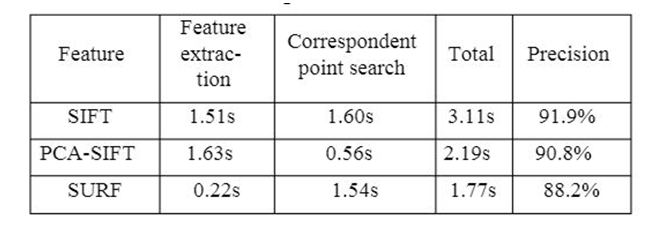
\includegraphics[scale=0.8]{./Figures/feature}
\caption{Precision and processing time of features}
\label{fig:1}
 		\end{figure}

Now we discuss about another application of capacitive sensors based on indoor localization. Capacitive sensing is that technique that tracking the conductive and non-conductive objects. This sensor is able to sense the 3D position of human and their interacting objects. 
 By using this technique, we can find the indoor location of the person by using human-body detection technique. It uses capacitive transducers which operate in 3 modes. But in this case, we use only 2 modes known as shunt mode or transmit mode for the detection of the body. Another scientist introduced the load operation mode. In this mode, human body acts as a potential-plate that is shown in Fig (a). Capacitances used in load mode are Cpb (plate-body capacitor), Cbg (body-ground capacitor) and Cpg (plate-ground capacitor). It is more suitable for deployment. For develop capacitive sensors based application, load operation mode is used.


\begin{figure}[h]
  		\centering
    		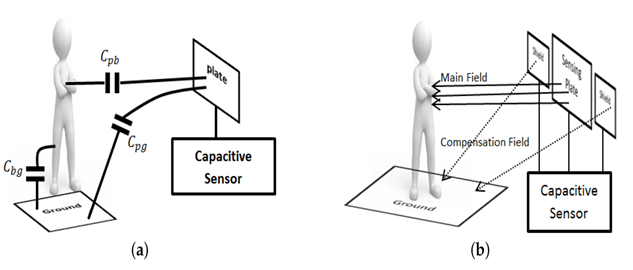
\includegraphics[scale=0.8]{./Figures/systemarchi}
\caption{System Architecture}
\label{fig:2}
 		\end{figure}
For develop this system, they also use some algorithms such K-NN (K-Nearest Neighbor), NB (Naive Byes), SVM (Support Vector Machine). To perform the experiment, they have a room in which they place sensor plates of 4cmX4cm. They deploy the sensors on the four sides of the room. After deploy the sensors, they used three algorithms as we explain above. These algorithms used to find the precision and recall of this indoor localization system. The precision and recall are given in table below:   

\begin{figure}[h]
  		\centering
    		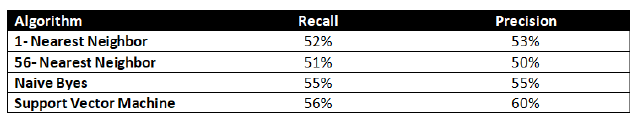
\includegraphics[scale=0.9]{./Figures/pr1}
\caption{Precision and recall of different algorithms}
\label{fig:3}
 		\end{figure}

They also perform this experiment with the room having sensor plates of 8cmX8cm. The results of precision and recall are different from the above results. They give better result than the above. The precision and recall of 8cmX8cm sensor plates are given in table below:  

\begin{figure}[h]
  		\centering
    		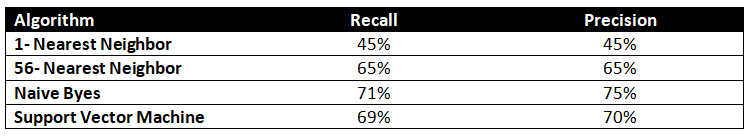
\includegraphics[scale=0.75]{./Figures/pr2}
\caption{Precision and recall of different algorithms}
\label{fig:4}
 		\end{figure}

They also perform this experiment with the room having sensor plates of 16cmX16cm. The results of precision and recall are also different from the above results. They give best result than all of the above. The precision and recall of 16cmX16cm sensor plates are given in table below:  

\begin{figure}[h]
  		\centering
    		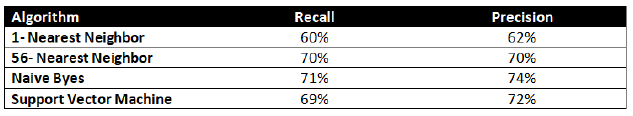
\includegraphics[scale=0.9]{./Figures/pr3}
\caption{Precision and recall of different algorithms}
\label{fig:5}
 		\end{figure}
Another most important technology, we discuss here. We have to discuss the indoor based localization using Wi-Fi. This application also tells the user to the position of the person where he stands. It also tells the indoor localization of the person. The patterns that connect the different access point of the Wi-Fi which is fixed to the various point and become unique. This pattern is called Wi-Fi finger printing. It consists of Received Signal Strength Indicator (RSSI) values and MAC Address data. RSSI values contain negative numbers. If RSSI values are closest to the zero (0) such as (-5) then It indicates that the signal strength is strong. 
The data set of this application consists of RSSI value and MAC address. The algorithms of machine learning also apply in this indoor based localization using Wi-Fi application. Due to the large data set. The fastest algorithm is used in this system. The algorithm which is used in this application is deep learning. Meanwhile, the machine learning algorithms such as k-NN, NB, SVM also used for this application. Their precision and recall also shown in table:

\begin{figure}[h]
  		\centering
    		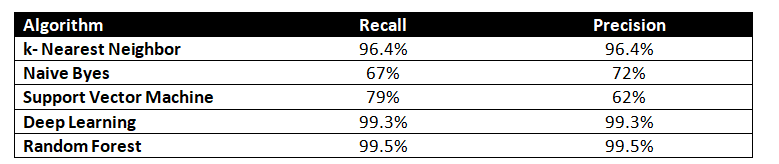
\includegraphics[scale=0.7]{./Figures/pr4}
\caption{Precision and recall of different algorithms}
\label{fig:6}
 		\end{figure}


\subsection{Comparison of Existing Work}
Here are the comparisons of some of them
\begin{figure}[h]
  		\centering
    		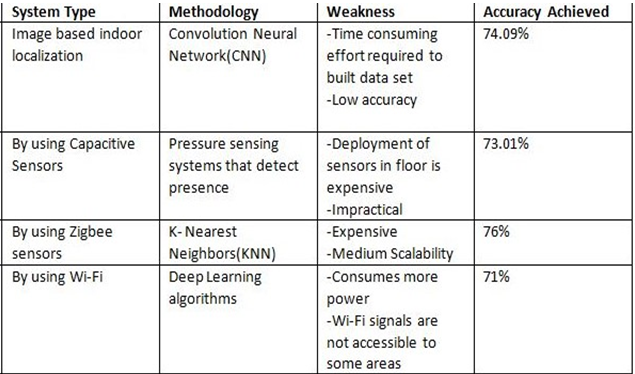
\includegraphics[scale=0.9]{./Figures/comparison}
\caption{Comparison between existing systems}
\label{fig:7}
 		\end{figure}

\subsection{Limitations of Existing System}
Here are some limitations of existing system which are as follows:
\begin{itemize}
\item In some systems, camera is required for indoor positioning which is not suitable for some users.
\item High cost and effort is required for the deployment of indoor localization.
\item Most of the existing systems have medium or low accuracy.
\item In image based indoor localization, time consuming effort is required for built data sets. 
\item It consumes more power.
\item There are some spots where Wi-Fi access points would be difficult to access.
\\\\
\end{itemize}

\subsection{Software Architecture}
Here is our software architecture:
\\\\
\begin{figure}[h]
  		\centering
    		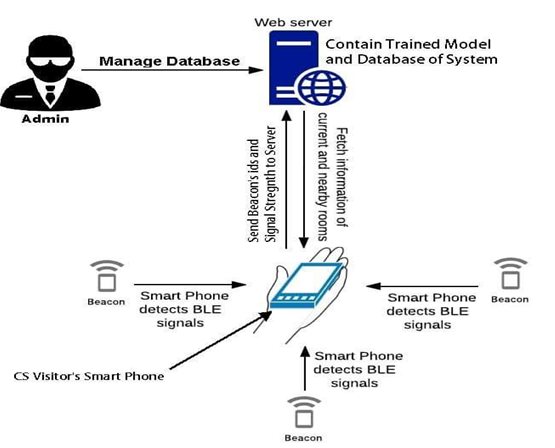
\includegraphics[scale=0.9]{./Figures/softarchi}
\caption{Software Architecture Diagram}
\label{fig:8}
 		\end{figure}


\section{Software Development Life Cycle Used}
To implement a project, one must have to follow some software development life cycle to deliver his project completely according to user requirements in time. By following a certain SDLC, a project developer feels so comfortable as he have specific tasks and time to implement project timely  which meets the user’s point of view. In our project, there are lots of fluctuations time by time. So, we decided to follow AGILE model.
\subsection{AGILE SDLC}
Agile SDLC model is a combination of incremental and iterative process models deals with customer requirements satisfaction and process adaptability by rapid delivery of working product to the customer. This model breaks the whole project in small modules. Do proper testing after completion of each module. Then deliver this working module to the customer and important stakeholders to satisfy them. If that module doesn’t meet their point of views properly or to which customer point of view as he didn’t explained in the document, then it has to be iterated to fulfill their new recommendations. And the other perspective is that if the customer wants to add some functionality in that particular module then a developer has to follow an incremental technique to add specific functionalities. 
To complete each deliverable module of the project, developer has to follow these steps
\begin{itemize}
\item Planning
\item Requirements Analysis
\item Design
\item Coding
\item Unit Testing and
\item Acceptance Testing
\end{itemize}

\begin{figure}[h]
\begin{center}
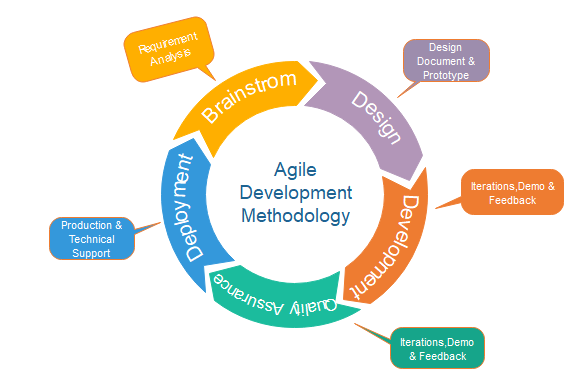
\includegraphics[scale=0.6]{agile}
\caption{Agile Development Methodology}
\label{fig:9}
\end{center}
\end{figure}
\subsection{Justification for AGILE SDLC}

These steps will justify that our project is based on agile methodology:
\begin{itemize}
\item All the requirement specifications and the scope of the project is strictly defined in our documentation but by the time, it may require some amendments, so they will change by ourselves.
\item Planning of time, design, implementation and testing is done.
\item Hardware and software parts of our project are specified into a work breakdown structure.
\item All the Modules of our project are divided in small pieces of time according to estimated time.
\item In model training module, we first use Weka and then following TensorFlow to meet the requirements; hence we followed an incremental and iterative model.
\item Do unit and acceptance testing after completion of each module.
\item Budget plan for our project is defined
\item We Add functionality of delay in Data Capturing application  which capture data after some seconds when a user change his indoor location.
\item Add restart functionality to restart scanning of Bluetooth devices once it stops which leads to incremental change in data capturing application.
\item Roles and responsibilities of team members vary according to the prescribed task and time limit.
\end{itemize}


\section{Requirement Analysis}
The most important section of system requirement specification document is requirement analysis. To start any project, anyone needs to know his system requirements. This section includes all the software, hardware functional requirements of our system, user interfaces, database diagram, use case diagram, use case tests and test cases. Basically, we will discuss all the specifications of our system.
\subsection{Hardware Functional Requirements}
\textbf{Deployment of BLE beacons}

Deployment of BLE beacons on the ceiling is the requirement to capture fingerprints of BLE beacons with different mobile devices. At what angle and at what part of the ceiling these beacons should display, all we get it know before their deployment.

\subsection{Software Functional Requirements}
\subsubsection{Data Capturing Application}
\textbf{Bluetooth scanning for nearby devices}

A scanning function is made in data capturing application to scan BLE beacon for nearby mobile devices. Devices who present/locate near a certain BLE beacon are being scanned.

\textbf{Capture RSSI values for nearby beacons}
BLE beacons Bluetooth range exists in a certain region and this region contain different mobile devices far and near to BLE beacon depending upon their indoor location. So, this function will capture RSSI fingerprints for all mobile devices which being scanned in that certain region.

\textbf{Add delay factor to capture FP’s}
 
Once fingerprints of certain mobile device have been captured at a particular location and by determining the indoor location, we provide room information through our application to a user’s mobile device. The user may change his indoor location after a while. To provide updated room information to the user we are making a delay function which captures user fingerprints after a certain time (seconds) and provide him updated information according to his room location.

\textbf{Automatic restart Bluetooth scanning for nearby devices once it stops}
 
Automatic restart scanning function will scan for BLE beacon nearby mobile devices once scanning has been stops, because in this way our system will able to automatically find coming and going devices in a particular region and provide rooms information accordingly.

\textbf{Generate .csv file for each BLE beacon}
 
After capturing the fingerprints of all devices with a single BLE beacon which lie in that certain region, this function will generate .csv file and RSSI values of all devices in that file.


\textbf{\textbf{\subsubsection{SmartGuide: Android Application}}}

The functional requirements of our system for User are as follows:

\textbf{Load trained model in Android app}

There is need to load machine learning trained model in our Android application to predict the room location of a particular person.

\textbf{Get the prediction of room from trained model}

When a trained model receives .csv file of a particular BLE beacon, it gives the particular roomID of that beacon to a mobile device which is receiving higher RSSI value from that BLE beacon.

\textbf{Allow user to know his indoor location}

This function will enable users to see their indoor location i.e. in which room they are.

\textbf{Fetch information of that particular room}

This function will send RoomID of a particular BLE beacon to the database from which room information in image, texts and audio format can be fetched.

\textbf{Provide information of the room to the user}

After fetching the information of a particular room, this function becomes enable and displayed that information on user mobile screen.

\textbf{Enable user to get information of nearby rooms}

This function allow users to see their nearby (left, right, front and back) rooms and textual and pictorial information about that rooms.
\\\\
The functional requirements of our system for Admin are as follows:

\textbf{Allow admin to SignUp for our application}

To use an Android application, in this case admin has to register on our application to add, update and delete records of certain data in our application.

\textbf{Provide account activation functionality to the admin}

Admin can login on another device; he has no restriction to use our application on a certain device. He may be login or logged out.

\textbf{Admin has all the records of data}

Admin has the ability to get all up-to-date records of data. Data can be of staff members, their visiting hours, room information, lab accessories and much more.

\textbf{Store information to database in images, audios and text format of rooms and their nearby rooms}

This function will store information about rooms in images, audios and text format in the database. Also, the information about nearby rooms of a certain room will also be stored by the admin in the database manually.

\textbf{Allow admin to edit or update the information about rooms}

When After sometime, the specifications and in formations about certain rooms and departments can be changed. So, this function will enable admin to update the information accordingly to provide up-to-date information to the user.

\textbf{Admin has all those functionalities which a user has}

Admin can see the information of a room and nearby rooms in any format provided in our application like user.

\subsection{Non Functional Requirements}
\textbf{Reliability}

Our project will be reliable .The user’s information will be kept confidential and there will be no worry of losing the information.

\textbf{Usability}

Our application will be usable for the users and easy to use.

\textbf{Maintainability}

This system will have the capability to adapt changes and amendments done in the database by the admin as the information of rooms will be updated or edited.

\textbf{Security}

Our Android application will work under potential risks. It will not be accessible by the malicious user or be crashed by external attacks.

\textbf{Recoverability}

In case of crash, our system information will recoverable

\textbf{Safety}

Optimize safety in the design, development, use and maintainability of the application.

\textbf{Reusability}

Our system will provide reusability factor to the visitors of the department.

\textbf{Performance}

To make a system which gives accurate and up-to-date information about rooms even a user change his indoor location after a while. This system will give results efficiently in small time.


\subsection{Use Case Diagram}
\begin{figure}[h]
\begin{center}
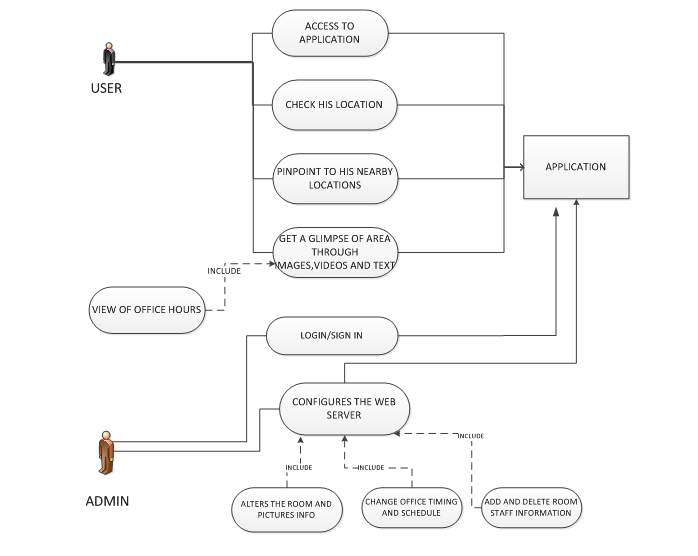
\includegraphics[scale=1.0]{usecase}
\caption{Usecase Diagram}
\label{fig:10}
\end{center}
\end{figure}
\clearpage
\subsection{Use Case Texts}

\begin{figure}[h]
\begin{center}
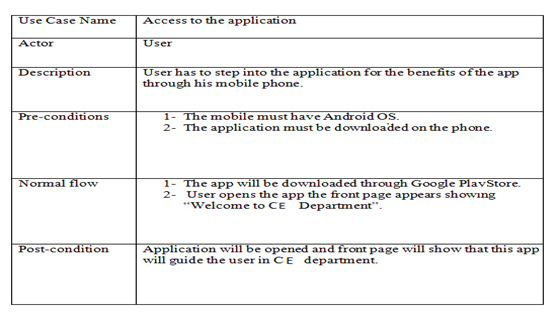
\includegraphics[scale=0.8]{uc1}
\caption{Usecase(1)}
\label{fig:11}
\end{center}
\end{figure}


\begin{figure}[h]
\begin{center}
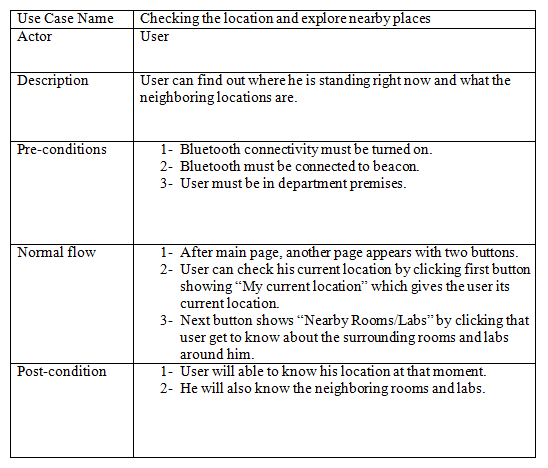
\includegraphics[scale=0.8]{uc2}
\caption{Usecase(2)}
\label{fig:12}
\end{center}
\end{figure}

\begin{figure}[h]
\begin{center}
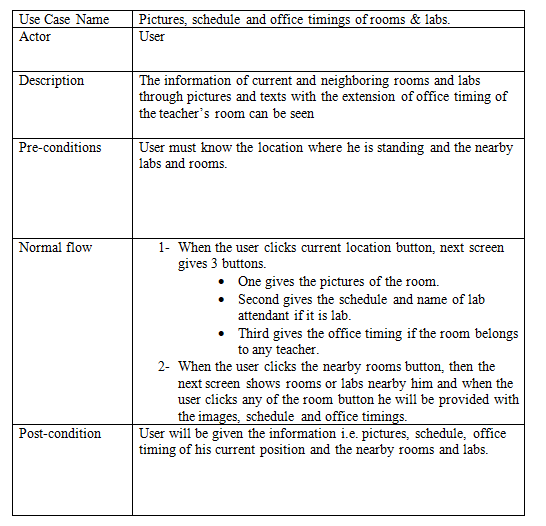
\includegraphics[scale=0.8]{uc3}
\caption{Usecase(3)}
\label{fig:13}
\end{center}

\end{figure}

\begin{figure}[h]
\begin{center}
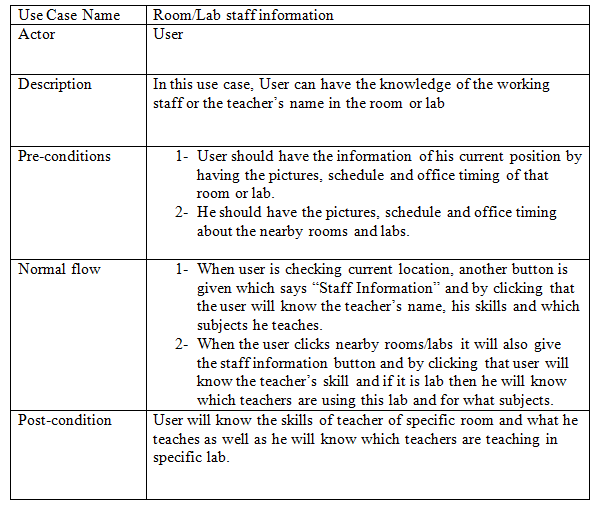
\includegraphics[scale=0.7]{uc4}
\caption{Usecase(4)}
\label{fig:14}
\end{center}
\end{figure}

\begin{figure}[h]
\begin{center}
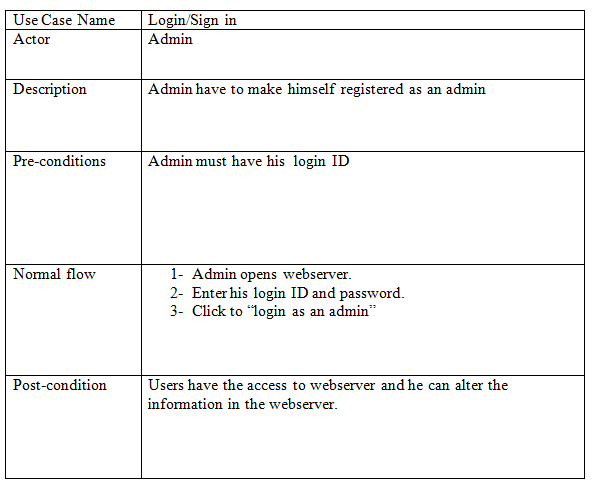
\includegraphics[scale=0.77]{uc5}
\caption{Usecase(5)}
\label{fig:15}
\end{center}
\end{figure}

\begin{figure}[h]
\begin{center}
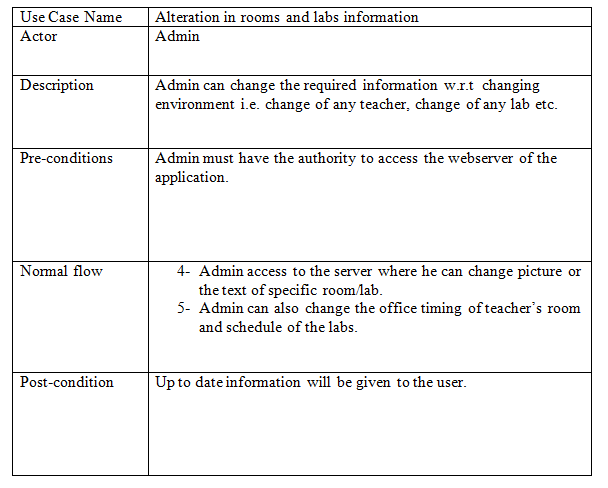
\includegraphics[scale=0.75]{uc6}
\caption{Usecase(6)}
\label{fig:16}
\end{center}
\end{figure}

\begin{figure}[h]
\begin{center}
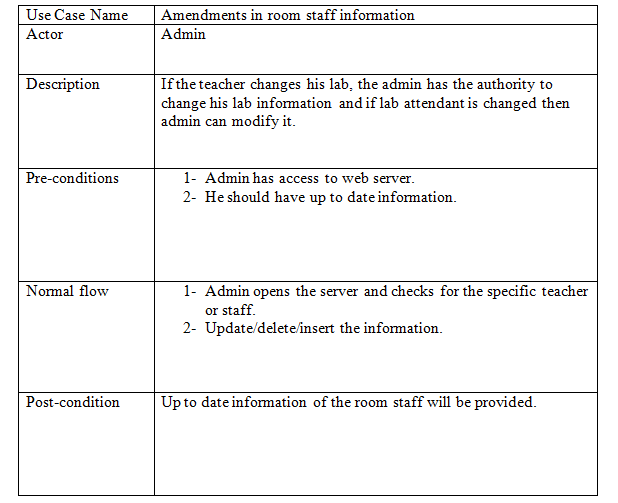
\includegraphics[scale=0.75]{uc7}
\caption{Usecase(7)}
\label{fig:17}
\end{center}
\end{figure}

\begin{figure}[h]
\subsection{Test Cases}
\begin{center}
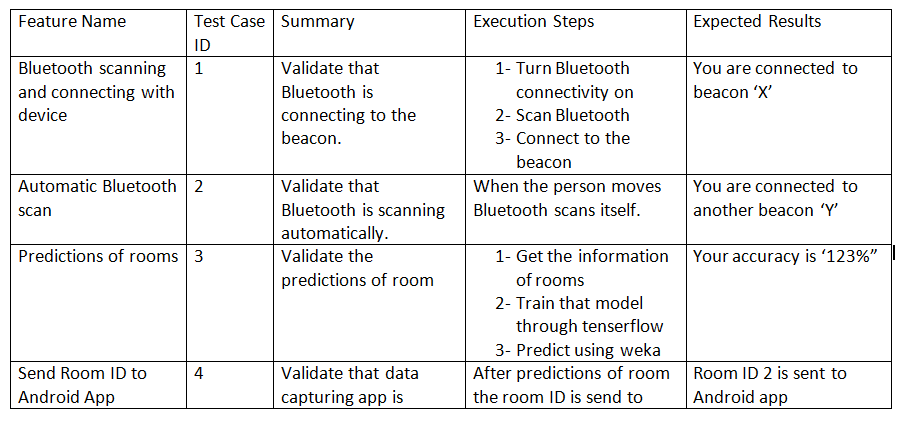
\includegraphics[scale=0.7]{tc1}
\caption{Testcase(1)}
\label{fig:18}
\end{center}
\end{figure}

\begin{figure}[h]
\begin{center}
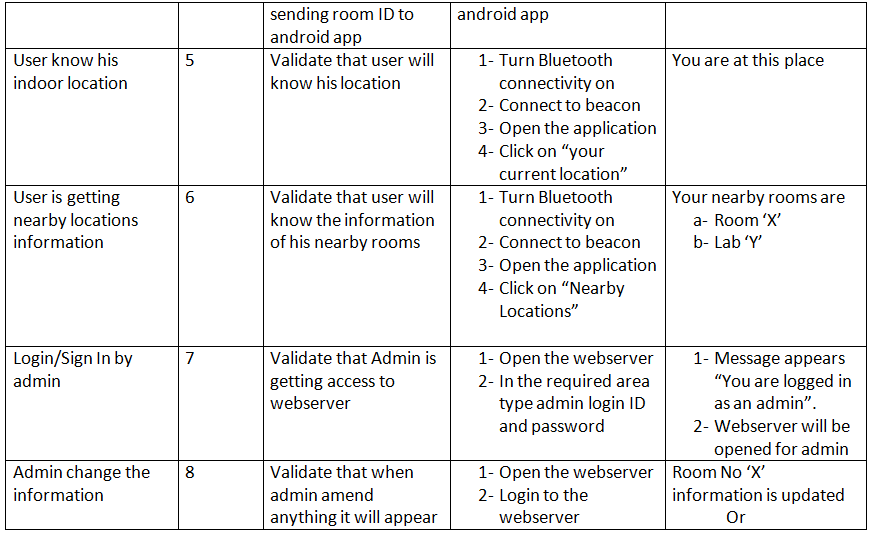
\includegraphics[scale=0.7]{tc2}
\caption{Testcase(2a)}
\label{fig:19}
\end{center}
\end{figure}

\begin{figure}[h]
\begin{center}
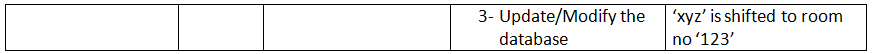
\includegraphics[scale=0.7]{tc3}
\caption{Testcase(2a)}
\label{fig:20}
\end{center}
\end{figure}


\clearpage


\section{Proposed System}

In our proposed system, an Android application provide guidance to campus isitors and make them familiar with department. Application will not only tell the current indoor location of user but also the information about current indoor location and nearby rooms in textual, image and audio formats. The location of the user is determined by taking predictions from the trained machine learning model on specific dataset. Dataset contains the RSSI fingerprints of BLE beacons  which we installed in the department, their MAC addressess and room rabels which we assigned to each room of the department in order to predict the class label. This dataset captured through a seperate Android Application named (BLE Scanner RSSI) which captures the RSSI values of nearby beacons from mobile device. 
Basically, there are two Android Applications, one is for the user through which we guide the user about the department through pictorial and textual information and the other application is for the admin who can do ammendments in the database. The database contains the information about rooms of the department i.e. the schedule of each lab for each class or the visiting hours and the specifcations of particular teacher and staff members. Semesterwise schedules, timetables and lab attendees varies timely in the department so this was must to update the information accordingly.
\\

\begin{figure}[h]
\begin{center}
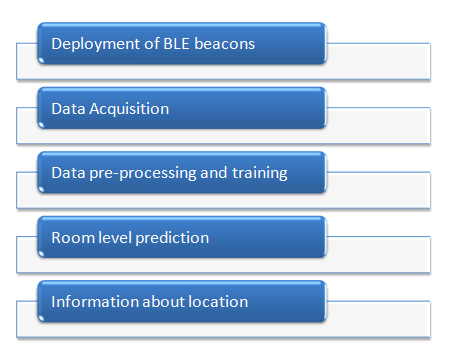
\includegraphics[scale=0.8]{proposedsystem}
\caption{Proposed System}
\label{fig:21}
\end{center}
\end{figure}

\clearpage
 \subsection{Deployment of BLE Beacons}
BLE beacons deployed in the experimental area which is Computer Engineering department of UET, Lahore. All the rooms of experimental area are assigned with a specific class label through which predict the location of the user's mobile device.Each room has its own lable range from L1 to L23. The detailed descritpion of the installment of BLE beacons in each room and floor of experimental area is shown in the figure below:

\begin{figure}[h]
\begin{center}
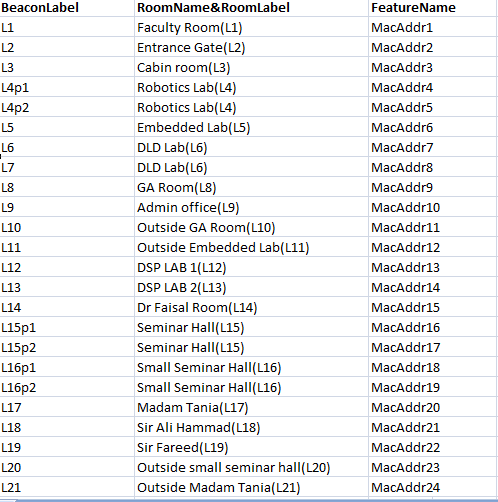
\includegraphics[scale=0.8]{beaconlabel}
\caption{Beacons labeling}
\label{fig:22}
\end{center}
\end{figure}

The placement of BLE beacons in the rooms, labs, corridors of both floors of the department is shown in previous chapter in detail.
\\

 \subsection{Data Acquisition}
BLE beacons broadcasts signals and these signals in the form of RSSI values will be captured at different positions by using Android application named(BLE Scanner RSSI) and then csv file will be generated which contains the MAC addresses of nearby BLE beacons from mobile device, class label and the RSSI fingerprints in the form of numerical values.

\begin{figure}
\begin{center}
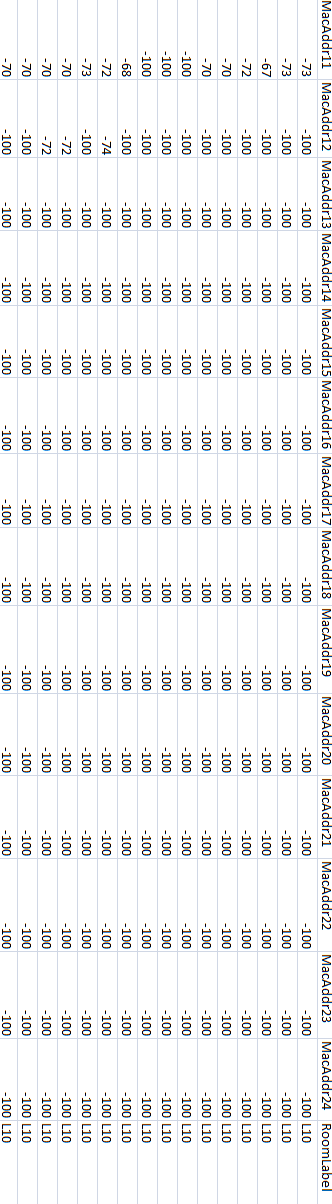
\includegraphics[scale=0.8]{dataeg}
\caption{Small portion of dataset}
\label{fig:23}
\end{center}
\end{figure}

\clearpage
 \subsection{Data Pre-processing and Training}
Pre-processing is done by replacing the null values of dataset by minimum signal strenth a device can recieve from BLE beacon according to our datset which is -100.Also, it includes the concatenation of thousand of csv files in one csv file to place our dataset at one place in file. Then this file is being used as an input to training algorithm, on which a classifier trains its model and make predictions. We trained this dataset by using machine learning algorithms i.e. knn, ann, random forest but artificial neural network gives us the high accuracy of training model as shown in figure. So, we decide to use ann as our selecetd model  and deployed this model on server.So, we can integrate our model to our Android application. 


\subsection{Room Level Prediction}
An Android application for common users will be developed that capture RSSI signals and send to server. Then trained model will take these values as input for the purpose of prediction of room and then send back the room label and its information to the user's application.
\subsection{Location Information}
Application will fetch information data of current room and nearby rooms in bith textual and pictorial formats from server and then display this information on the screen.







 % Experiment 1

%% Chapter 2

\chapter{Results and Discussions} % Write in your own chapter title
\label{Chapter5}
\lhead{Chapter 5. \emph{Results and Discussions}} % Write in your own chapter title to set the page header

As we have  to predict the indoor location of the user, we gathered our dataset by capturing RSSI fingerprints using our data capturing application which we further use to train our machine learning model.To train our machine learning model, we use three different machine learning algorithms. Firstly knn, which we used for supervised machine learning problem i.e.multiclassification problem. After tuning hyper-parameters of knn, it gives us accuracy of 90.04 while measuring Euclidean distance and of 90.03 while measuring Manhattan distance as shown in the figure(a). The impact of different number of weights on accuracy score is shown in figure(b).

\begin{center}
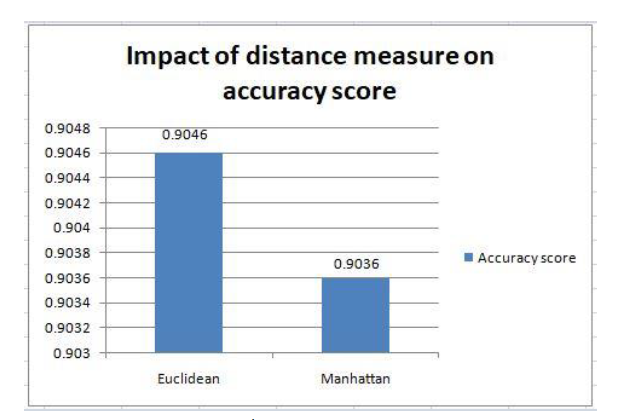
\includegraphics[scale=0.78]{dis}
\\Figure(a)
\end{center}

\begin{center}
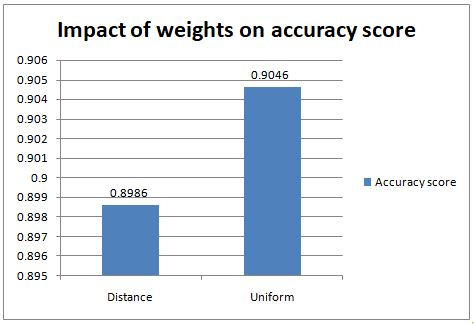
\includegraphics[scale=0.97]{weights}
\\Figure(b)
\end{center}

Secondly, we choose random forest algorithm which works on the principle of random creation of decision trees and gives the final prediction by polling the score of all decision trees for multiclassification problems. We tuned random forest algorithm on different hyper-parameters i.e. number of decision trees, maximum number of splits and nodes. The best combination of setting these parameters gives us the trainng accuracy of 95.33 and testing accuracy of 90.1. The imapct of different number of trees and random number of states is shown in the figures(c and d). The importance of each feature of our dataset is shown in figure(d).


\begin{center}
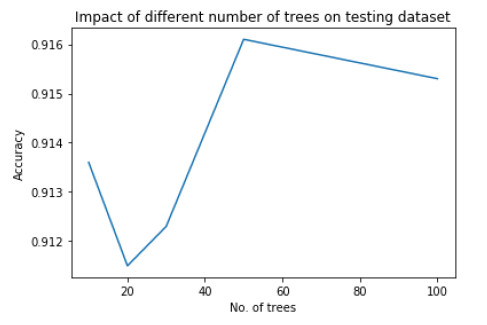
\includegraphics[scale=0.9]{rftree}
\\Figure(c)
\end{center}

\begin{center}
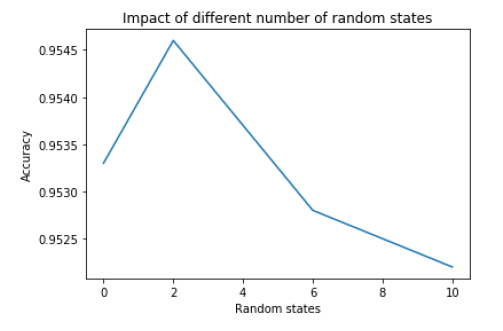
\includegraphics[scale=0.9]{rfrs}
\\Figure(d)
\end{center}
\begin{center}
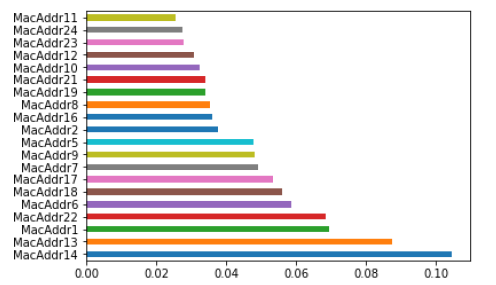
\includegraphics[scale=0.85]{rffeature}
\\Figure(e)
\end{center}

For the better prediction of the indoor location of the user, we thirdly use neural networks in which we use 2-layered neural network for our multi-classification problem.The input layer consists of input neurons. Those neurons transmit data to the next layer, which in turn sends the output neurons to the output layer. To implement this algorithm, we have to find the best values for parameters at which accuracy score is maximum. For this purpose, we use GridsearchCV function to test for all possible combinations. Here are the results of impact of optimizations algorithms on accuracy score.
\begin{center}
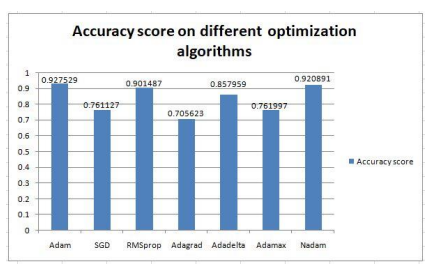
\includegraphics[scale=1.0]{optalgos}
\end{center}

We also tune activation functions { 'relu', 'tanh', 'sigmoid', ‘linear’}. All of them gave same accuracy score.Hence, after checking the impact of choosing different values of parameters on accuracy score, we find out that best combination has following values:
\begin{itemize}
\item Batch size: 40
\item Epochs: 250
\item Optimization Algorithm: ‘Adam’
\item Weight Initialization Methods: ‘uniform’
\item Activation Function: ‘relu’ for hidden layer and ‘sigmoid’ for output layer
\item Number of Neurons for hidden layer: 27
\end{itemize}
So,we conclude that on the basis of accuracy, precision and recall score for k-NN, Random forest and ANN. It is clear that ANN has highest accuracy, precision and recall score. Hence, ANN is our selected mode.
\pagebreak

\section{Graphs}

The  accuracy, precision and recall graph of knn is as follows:
\begin{figure}[h]
  		\centering
    		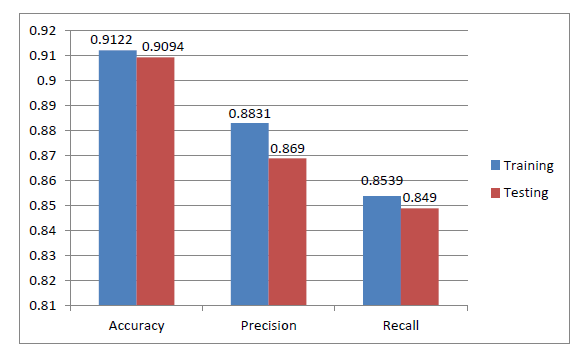
\includegraphics[scale=0.85]{./Figures/knncmgraph}
 		\end{figure}


The  accuracy, precision and recall graph of ann is as follows:

\begin{figure}[h]
  		\centering
    		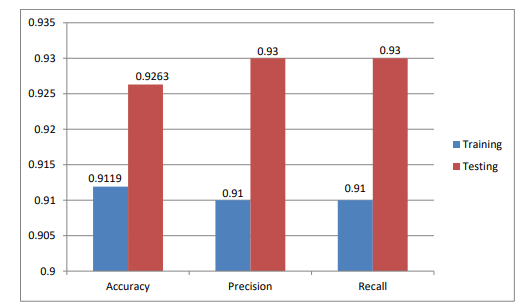
\includegraphics[scale=0.9]{./Figures/cmgraph}
 		\end{figure}

\pagebreak
\section{Confusion Matrix}

For the better prediction of the algorithms, we draw confusion matrix of the algorithims. The confusion matrix for knn is shown in the Figure(a) . As it is a multi-classification problem, it is a little bit different from binary classification. For example: ‘L1’ row shows that out of total samples in test data where data is labeled as ‘L1’, 92 instances were correctly classify, while 4 samples were wrongly predicted as ‘L9’.
\\\\
\begin{figure}[h]

  		\centering
    		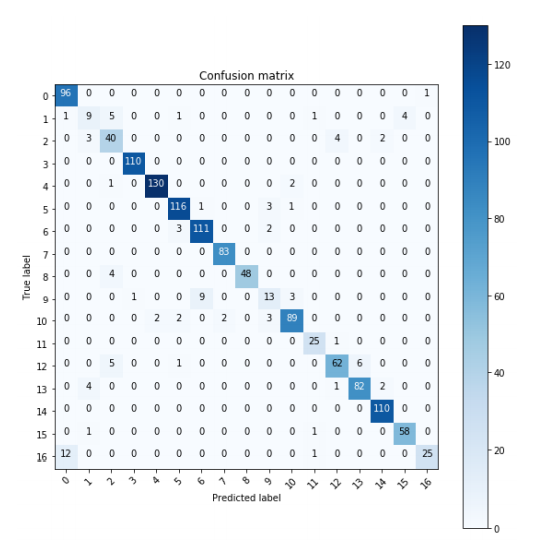
\includegraphics[scale=0.7]{./Figures/cm}
\\Figure(a)
 		\end{figure}


The confusion matrix for ann algorithm is shown in the Figure(b). As we use label encoder, so it encode classes ranges from 0 to 16. Here is the actual sequence, it means ‘L1’ encode to 0, ‘L10’ encode to 1 and so on:
\\\\
%['L1','L10','L11','L12','L13','L15','L16','L19','L2','L20','L21','L3','L4','L5','L6','L8','L9']
\begin{figure}[h]

  		\centering
    		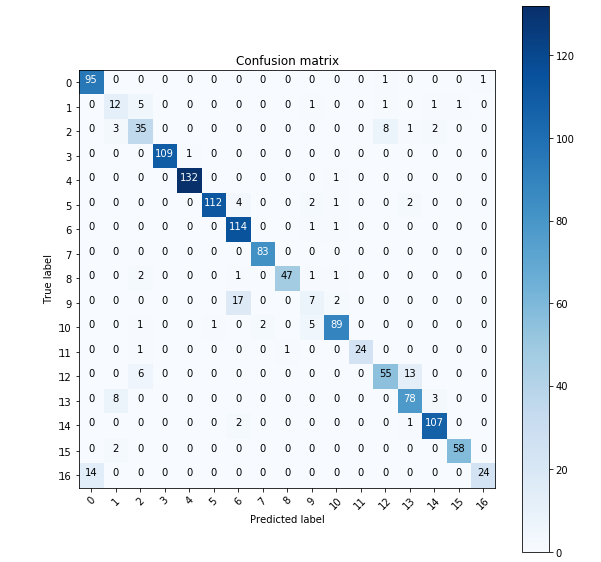
\includegraphics[scale=0.7]{./Figures/cmann}
\\Figure(b)
 		\end{figure}


 % Experiment 2

%% Chapter 2

\chapter{Results and Discussions} % Write in your own chapter title
\label{Chapter5}
\lhead{Chapter 5. \emph{Results and Discussions}} % Write in your own chapter title to set the page header

As we have  to predict the indoor location of the user, we gathered our dataset by capturing RSSI fingerprints using our data capturing application which we further use to train our machine learning model.To train our machine learning model, we use three different machine learning algorithms. Firstly knn, which we used for supervised machine learning problem i.e.multiclassification problem. After tuning hyper-parameters of knn, it gives us accuracy of 90.04 while measuring Euclidean distance and of 90.03 while measuring Manhattan distance as shown in the Figure 5.1. 
\begin{figure}[h]
\begin{center}
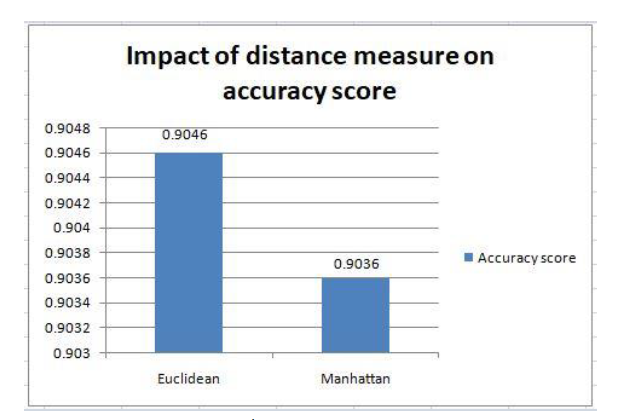
\includegraphics[scale=0.78]{dis}
\caption{Impact of distance measure on accuracy score}
\label{fig:1}
\end{center}
\end{figure}
Secondly, we choose random forest algorithm which works on the principle of random creation of decision trees and gives the final prediction by polling the score of all decision trees for multiclassification problems. We tuned random forest algorithm on different hyper-parameters i.e. number of decision trees, maximum number of splits and nodes. The best combination of setting these parameters gives us the trainng accuracy of 95.33 and testing accuracy of 90.1. The imapct of different number of trees  is shown in the Figure 5.2. 

\begin{figure}[h]
\begin{center}
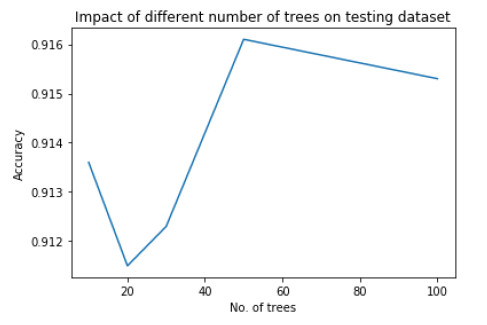
\includegraphics[scale=0.9]{rftree}
\caption{Impact of different number of trees on testing dataset}
\label{fig:2}
\end{center}
\end{figure}


For the better prediction of the indoor location of the user, we thirdly use neural networks in which we use 2-layered neural network for our multi-classification problem.The input layer consists of input neurons. Those neurons transmit data to the next layer, which in turn sends the output neurons to the output layer. To implement this algorithm, we have to find the best values for parameters at which accuracy score is maximum. For this purpose, we use GridsearchCV function to test for all possible combinations. Here are the results of impact of optimizations algorithms on accuracy score.

\begin{figure}[h]
\begin{center}
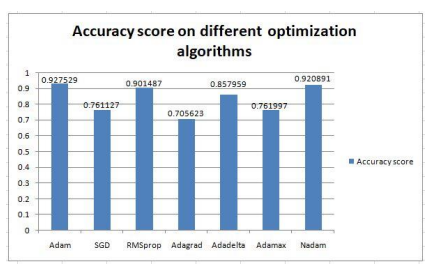
\includegraphics[scale=1.0]{optalgos}
\caption{Accuracy score on different optimization algorithms}
\label{fig:3}
\end{center}
\end{figure}

We also tune activation functions { 'relu', 'tanh', 'sigmoid', ‘linear’}. All of them gave same accuracy score.Hence, after checking the impact of choosing different values of parameters on accuracy score, we find out that best combination has following values:
\begin{itemize}
\item Batch size: 40
\item Epochs: 250
\item Optimization Algorithm: ‘Adam’
\item Weight Initialization Methods: ‘uniform’
\item Activation Function: ‘relu’ for hidden layer and ‘sigmoid’ for output layer
\item Number of Neurons for hidden layer: 27
\end{itemize}
So,we conclude that on the basis of accuracy, precision and recall score for k-NN, Random forest and ANN. It is clear that ANN has highest accuracy, precision and recall score. Hence, ANN is our selected mode.
\pagebreak

\section{Graphs}

The  accuracy, precision and recall graph of knn is as follows:
\begin{figure}[h]
  		\centering
    		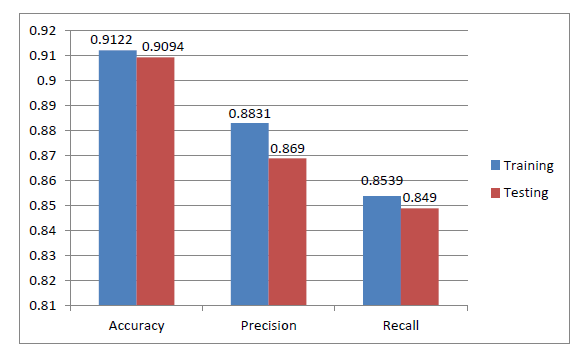
\includegraphics[scale=0.85]{./Figures/knncmgraph}
\caption{Accuracy, precision and recall graph of knn on training and testing sets}
\label{fig:4}
 		\end{figure}

The  accuracy, precision and recall graph of ann is as follows:

\begin{figure}[h]
  		\centering
    		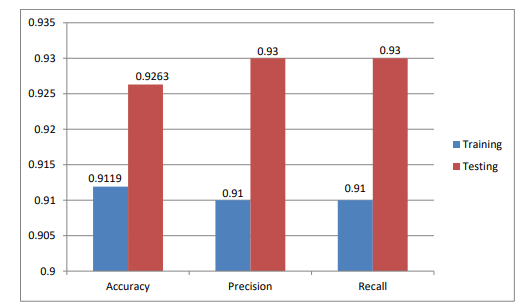
\includegraphics[scale=0.9]{./Figures/cmgraph}
\caption{Accuracy, precision and recall graph of ann on training and testing sets}
\label{fig:5}
 		\end{figure}

\pagebreak
\section{Confusion Matrix}

For the better prediction of the algorithms, we draw confusion matrix of the algorithims. The confusion matrix for knn is shown in the Figure(a) . As it is a multi-classification problem, it is a little bit different from binary classification. For example: ‘L1’ row shows that out of total samples in test data where data is labeled as ‘L1’, 92 instances were correctly classify, while 4 samples were wrongly predicted as ‘L9’.
\\\\
\begin{figure}[h]

  		\centering
    		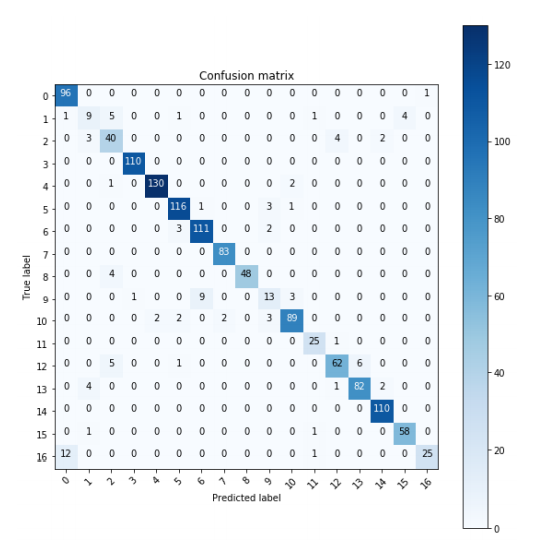
\includegraphics[scale=0.7]{./Figures/cm}
\caption{Confusion matrix for the evaluation of knn}
\label{fig:6}
 		\end{figure}


The confusion matrix for ann algorithm is shown in the Figure(b). As we use label encoder, so it encode classes ranges from 0 to 16. Here is the actual sequence, it means ‘L1’ encode to 0, ‘L10’ encode to 1 and so on:
\\\\
%['L1','L10','L11','L12','L13','L15','L16','L19','L2','L20','L21','L3','L4','L5','L6','L8','L9']
\begin{figure}[h]

  		\centering
    		\includegraphics[scale=0.7]{./Figures/cmann}
\caption{Confusion matrix for the evaluation of ann}
\label{fig:7}
 		\end{figure}


 % Results and Discussion

%% Chapter 1

\chapter{Thesis Contribution and Future Work} % Write in your own chapter title
\label{Chapter1}
\lhead{Chapter 1. \emph{Introduction}} % Write in your own chapter title to set the page header

\section{Introduction}
As we have discussed all the parameters in this thesis such as introduction, methodology, implementation, results etc. After results and experiments, this proposed system motivates us to do some more work on it. So, in this chapter, we will discuss the work that we will do in future. But before discuss the future work, we will discuss about the thesis contribution.

\subsection{Thesis Contribution}
 According to previous research papers, indoor localization based applications using different techniques. Most of the applications based on Wi-Fi. Image based indoor localization, capacitive sensors, Zigbee Wi-Fi are previous technique for indoor localization. In our research work, we have to make an android application which tells the indoor location of the user using BLE beacons. There are some points which describe that what our contribution in thesis which is as follows:

\begin{itemize}
\item Bluetooth beacons are much more compatible than other devices such as Wi-Fi, Image based indoor localization, capacitive sensors, Zigbee Wi-Fi.
\item BLE beacon consumes less energy. It is light weight and cheaper than Wi-Fi signals. BLE beacons are usually battery powered, which are more flexible. It is easier to sense the signals. 
\item Our system is much more compatible than other indoor based localization application.
\item Our system provides much more reliability, maintainability, security and safety, reusability than other indoor based localization applications.
\item It gives better performance than other indoor based localization applications.
\item Our System is user friendly and easy to use.
\item Our system well-defined the location of the user than other indoor based localization applications.
\item Our system also tells the entire information of the room in which user is present which other indoor based localization applications not tell.
\item It also tells the entire information of nearby room which other indoor based localization applications not tell.
\item Our system tells the information of the rooms and nearby rooms in the form of texture, pictures and audio format.
\item Our proposed system supports the mobile devices such as  tablets and smart phones
\item Our proposed system supports the Android OS (Operating System).

\end{itemize}

\subsection{Future Work}
To improve the accuracy and performance of this purposed system, we want to do further work on them. We also want to do this project on commercial level. Actually the idea of our project is world changing. But due to limited resources, we implement this idea on a specific workspace. Here we discuss some points in which we will implement in the future.\

\begin{itemize}
\item First of all, we want to develop an algorithm which gives more precise accuracy than previous algorithms such as k-NN, ANN and RF (Random Forest). 
\item We want to work on a big data set such as data set of all over university. For this purpose we will capture the data of all over the university.
\item We will develop an application with different database. Actually, the database of one department of the university includes rooms, room members and office hours of the room members. But when we will work on the university, the database is different.
\item For our proposed system, we use online database. But in future, we want to make an offline database. So that, when users install the app in the mobile, the overall data is also installed in the mobile.
\item We will develop an android application for our CSE department, UET Lahore. But in future we will make this application for whole university.
\item If we will have more resources in the future, we will make this system for other places such as hospitals, offices, shopping malls and other universities
\end{itemize}.



 % Conclusion

%% ----------------------------------------------------------------
% Now begin the Appendices, including them as separate files

\addtocontents{toc}{\vspace{2em}} % Add a gap in the Contents, for aesthetics

%\appendix % Cue to tell LaTeX that the following 'chapters' are Appendices

%% Appendix A

\chapter{Introduction to Latex}
\label{AppendixA}
\lhead{Appendix A. \emph{Introduction to Latex}}

The material provided in this appendix is taken from \\
\href{http://www.sunilpatel.co.uk/thesistemplate.php}{\texttt{http://www.sunilpatel.co.uk/thesistemplate.php}}

\section{Learning \LaTeX{}}

\LaTeX{} is not a WYSIWYG (What You See is What You Get) program, unlike word processors such as Microsoft Word or Corel WordPerfect. Instead, a document written for \LaTeX{} is actually a simple, plain text file that contains \emph{no formatting}. You tell \LaTeX{} how you want the formatting in the finished document by writing in simple commands amongst the text, for example, if I want to use \emph{italic text for emphasis}, I write the `$\backslash$\texttt{emph}\{\}' command and put the text I want in italics in between the curly braces. This means that \LaTeX{} is a ``mark-up'' language, very much like HTML.

\subsection{A (not so short) Introduction to \LaTeX{}}

If you are new to \LaTeX{}, there is a very good eBook -- freely available online as a PDF file -- called, ``The Not So Short Introduction to \LaTeX{}''. The book's title is typically shortened to just ``lshort''. You can download the latest version (as it is occasionally updated) from here:\\
\href{http://www.ctan.org/tex-archive/info/lshort/english/lshort.pdf}{\texttt{http://www.ctan.org/tex-archive/info/lshort/english/lshort.pdf}}

It is also available in several other languages. Find yours from the list on this page:\\
\href{http://www.ctan.org/tex-archive/info/lshort/}{\texttt{http://www.ctan.org/tex-archive/info/lshort/}}

It is recommended to take a little time out to learn how to use \LaTeX{} by creating several, small `test' documents. Making the effort now means you're not stuck learning the system when what you \emph{really} need to be doing is writing your thesis.

\subsection{A Short Math Guide for \LaTeX{}}

If you are writing a technical or mathematical thesis, then you may want to read the document by the AMS (American Mathematical Society) called, ``A Short Math Guide for \LaTeX{}''. It can be found online here:\\
\href{http://www.ams.org/tex/amslatex.html}{\texttt{http://www.ams.org/tex/amslatex.html}}\\
under the ``Additional Documentation'' section towards the bottom of the page.

\subsection{Common \LaTeX{} Math Symbols}
There are a multitude of mathematical symbols available for \LaTeX{} and it would take a great effort to learn the commands for them all. The most common ones you are likely to use are shown on this page:\\
\href{http://www.sunilpatel.co.uk/latexsymbols.html}{\texttt{http://www.sunilpatel.co.uk/latexsymbols.html}}

You can use this page as a reference or crib sheet, the symbols are rendered as large, high quality images so you can quickly find the \LaTeX{} command for the symbol you need.



\subsection{Figures}

There will hopefully be many figures in your thesis (that should be placed in the `Figures' folder). The way to insert figures into your thesis is to use a code template like this:
\begin{verbatim}
\begin{figure}[htbp]
  \centering
    \includegraphics[width = 1.5in]{./Figures/uet_logo.pdf}
    \rule{35em}{0.5pt}
  \caption{The UET Laore logo.}
  \label{fig:uet_logo}
\end{figure}
\end{verbatim}
Also look in the source file. Putting this code into the source file produces the picture of the UET logo that you can see in the figure below.

\begin{figure}[htbp]
	\centering
		\includegraphics[width = 1.5in]{./Figures/uet_logo.pdf}
		\rule{35em}{0.5pt}
	\caption{The UET Laore logo.}
	\label{fig:uet_logo}
\end{figure}

Sometimes figures don't always appear where you write them in the source. The placement depends on how much space there is on the page for the figure. Sometimes there is not enough room to fit a figure directly where it should go (in relation to the text) and so \LaTeX{} puts it at the top of the next page. Positioning figures is the job of \LaTeX{} and so you should only worry about making them look good!

Figures usually should have labels just in case you need to refer to them (such as in figure \ref{fig:uet_logo}). The `$\backslash$\texttt{caption}' command contains two parts, the first part, inside the square brackets is the title that will appear in the `List of Figures', and so should be short. The second part in the curly brackets should contain the longer and more descriptive caption text.

The `$\backslash$\texttt{rule}' command is optional and simply puts an aesthetic horizontal line below the image. If you do this for one image, do it for all of them.

The \LaTeX{} Thesis Template is able to use figures that are either in the PDF or JPEG file format. It is recommended that you read this short guide on how to get the best out of figures in \LaTeX{}, available here:\\
\href{http://www.sunilpatel.co.uk/texhelp5.html}{\texttt{http://www.sunilpatel.co.uk/texhelp5.html}}

Though it is geared more towards users of Mac and OS X systems, much of the advice applies to creating and using figures in general. It also explains why the PDF file format is preferred in figures over JPEG.

\subsection{Typesetting mathematics}

If your thesis is going to contain heavy mathematical content, be sure that \LaTeX{} will make it look beautiful, even though it won't be able to solve the equations for you.

The ``Not So Short Introduction to \LaTeX{}'' (available \href{http://www.ctan.org/tex-archive/info/lshort/english/lshort.pdf}{here}) should tell you everything you need to know for most cases of typesetting mathematics. If you need more information, a much more thorough mathematical guide is available from the AMS called, ``A Short Math Guide to \LaTeX{}'' and can be downloaded from:\\
\href{ftp://ftp.ams.org/pub/tex/doc/amsmath/short-math-guide.pdf}{\texttt{ftp://ftp.ams.org/pub/tex/doc/amsmath/short-math-guide.pdf}}

There are many different \LaTeX{} symbols to remember, luckily you can find the most common symbols \href{http://www.sunilpatel.co.uk/latexsymbols.html}{here}. You can use the web page as a quick reference or crib sheet and because the symbols are grouped and rendered as high quality images (each with a downloadable PDF), finding the symbol you need is quick and easy.

You can write an equation, which is automatically given an equation number by \LaTeX{} like this:
\begin{verbatim}
\begin{equation}
E = mc^{2}
  \label{eqn:Einstein}
\end{equation}
\end{verbatim}

This will produce Einstein's famous energy-matter equivalence equation:
\begin{equation}
E = mc^{2}
\label{eqn:Einstein}
\end{equation}

All equations you write (which are not in the middle of paragraph text) are automatically given equation numbers by \LaTeX{}. If you don't want a particular equation numbered, just put the command, `$\backslash$\texttt{nonumber}' immediately after the equation.


\section{Sectioning and Subsectioning}

You should break your thesis up into nice, bite-sized sections and subsections. \LaTeX{} automatically builds a table of Contents by looking at all the `$\backslash$\texttt{chapter}$\{\}$', `$\backslash$\texttt{section}$\{\}$' and `$\backslash$\texttt{subsection}$\{\}$' commands you write in the source.

The table of Contents should only list the sections to three (3) levels. A `$\backslash$\texttt{chapter}$\{\}$' is level one (1). A `$\backslash$\texttt{section}$\{\}$' is level two (2) and so a `$\backslash$\texttt{subsection}$\{\}$' is level three (3). In your thesis it is likely that you will even use a `$\backslash$\texttt{subsubsection}$\{\}$', which is level four (4). Adding all these will create an unnecessarily cluttered table of Contents and so you should use the `$\backslash$\texttt{subsubsection$^{*}\{\}$}' command instead (note the asterisk). The asterisk ($^{*}$) tells \LaTeX{} to omit listing the subsubsection in the Contents, keeping it clean and tidy.
	% Appendix Title

\newpage
\chapter{Introduction}
\section{Overview Of Project}
Advertising plays a critical role in marketing of a product. The ads released by the company represents the product and if not attractive enough or contain any factor disliked by the customer then its reputation can be damaged in an instant. Therefore, one needs to be careful about the customer’s likeness in order to avoid the financial and reputational damage. Every year, a company allocates a specific amount of marketing budget for the evaluation of advertisements realizing its importance in the promotion of a product. So, in order to provide a better and more reliable way to get customer’s feedback and to detect the effectiveness of an ad, an EEG based system for advertisement’s impact assessment will be established using machine learning techniques for automation of advertisement review analysis. In the proposed system, a low cost EEG headset i.e. Neurosky Mindwave Mobile will be used to collect the brain signals including different brain waves like alpha, beta, gamma and delta each of them being specific to a certain kind of activity of the subject viewing advertisements that aims in providing the statistics of the advertisement's impact and the likelihood of a person purchasing the advertised product. Different features like attention and meditation which are used to characterize the experience of the consumer will be extracted by continuously monitoring and analyzing the consumers’ brain activity. Then classification will be performed and results will be generated whether the customer liked or disliked the specific ad. This analysis will help us provide the statistical trend for a certain kind of advertisement on the basis of various factors. It will greatly help the marketing sector of multinational companies to improve their advertising campaign according to the feedback collected from different customers which will bring a revolutionary change in how they perceive their brand.
\section{Background}
Since the very beginning, marketers strive for understanding consumers preferences and what they were thinking in order to make their ads more productive by using traditional approaches. These techniques known as direct observation method include asking customers what they think and collecting data through surveys and focus groups and then its analysis, which require more manpower and has longer cycle in order to accomplish the results. Moreover, asking the person's review is unreliable because may be most of the time the person is not telling his/her genuine remarks. It is also more laborious, time consuming and less accurate. On the other hand, advertisements are considered very important nowadays as a huge amount of money is being spent on them globally. If we take a look at its global statistics, the latest Dentsu Aegis Network Ad Spend forecasts show in 2019 the growth will increase by 3.8\%, amounting to US\$625 billion \cite{b1}. If we look back in year 2016, the advertising global spending was worth \$500billion\cite{b2}.And if marketing expense i.e. research, marketing,etc.then the total worth of industry
becomes \$965 billion. Global advertising spending from 2010 to 2018 (in billion U.S.dollars) is shown in Figure 1 \cite{b3} below:

\begin{figure}[htbp]
\centerline{\includegraphics[scale=0.6]{Figure1.png}}
\caption{Global advertising spending from 2010 to 2019 (in billion U.S. dollars)}
\label{Figure 1}
\end{figure}
Therefore, considering the importance of ads, one cannot rely on such traditional techniques and need some advancement.\par
Some current assessment methods also contains indirect inference from observing changes in customer’s behavior after releasing the advertisement which requires a lot of time and also ad campaign has to be launched beforehand which most probably means cost is already at risk. Similarly some techniques like interpreting person's facial expression and inspecting thoroughly their hand–eye coordination are also applied. All these methods have some drawbacks like some are time consuming while other are ambiguous and may lead one to take inappropriate actions to reach the goal. Whereas, directly collecting the EEG brain waves in order to get the customer’s feedback will be less time consuming and will yield more accurate result.

\section{Motivation}
In today’s world, advertising is a huge business. It gives important information in productive and cost-effective way regarding the services and products and is a powerful tool of competition. Therefore, advertising helps the economy to function smoothly by facilitating the entry of advanced and unfamiliar products and new brands into the market. As we already know that consumer’s opinion plays a major role in making an advertisement . Keeping that in mind, Some major aspects that motivated us to opt this project are:

\begin{itemize}
\item The advertising industry in Pakistan is growing anually at a rate of 10-12pc and it worth \$650 million because of continuously emerging urban middle class and increase in consumerism, purchasing power, and an expanding economy \cite{b2}. So, we need some reliable methods to make our advertisements better and avoid the financial risk. 
\item In Pakistan, advertising sector is frequently criticized because of its lack of creativity and detest of the consumers. The need of the hour is to create productive ads according to customer’s likeness as consumer confidence matters the most \cite{b4}.
\item Nowadays, advertising campaigns are represented by creative and productive and ideas rather than expensive brand endorsements. What matters is the material that clicks in customer's minds. Current campaign shows that communications is the important part and gone are the days when you could just make consumer accept an idea by continuously showing it. 
\item Currently, Pakistan is a hot  market for multinationals as it is growing very rapidly and that is why they are increasing the spend on advertsement. TV remains the biggest medium for media spend in Pakistan with Rs30 billion spending. As the country is spending so much in advertising, the ads must be according to consumer’s likeness to reduce the risk of loss.
\end{itemize}
\newpage
\chapter{Objectives}
The use of brain signals to study one’s response is a very effective way for analysis. It gives a proper insight to what is one’s behavior and what decision one will make regarding something. 

\section{Industry Objectives}
The success of any product highly depends on its marketing and advertisement analysis is very important in brand marketing. Every year companies set a specific marketing budget for their advertising campaign. People are asked to fill questionnaires in order to record their response regarding their brand or a particular advertisement for their brand. However, such responses are mostly ambiguous, biased and does not help in a fruitful assessment. To overcome this problem, our aim is to use the technique of neuro-marketing and automate the consumer feedback mechanism for analysis of any kind\cite{b6}. It is supposed to guide the marketers to the right product designs and ad messages to boost sales. Many companies like Hyundai, Google, Walt Disney, Microsoft, Chevron etc\cite{b5}. Few of the industrial objectives are as follows:

\begin{itemize}
\item The system must allow the analysts to fill in the gaps left by traditional marketing methods.
\item It must help the marketing analysts understand the consumer preferences in order to improve brand quality, advertisements, packaging etc.
\item Our project should focus on the study of brain responses to marketing stimuli which will revolutionize marketing sector of industries.
\item It must be so economical causing the industries to save on their marketing expenses by recording consumers’ response in an effective and efficient way\cite{b7}.
\item System must cut off losses of industries in marketing sector, by making them predict consumers’ response using advanced techniques accurately.
\item Main aim of our project is to develop a system that is cost effective and error free than the previously designed systems which will eventually lead the industrial field to progress\cite{b8}.
\item It must help the industrial sector to make necessary changes wherever required in the product or advertisement beforehand by analyzing consumers’ behavior.
\end{itemize}

\section{Research Objectives}
These objectives involve, a comprehensive study of all the research done in the system’s development field and then on its basis, developing a system that can be able to acquire brain signals and classify them in order to predict the results accurately and in turn should be better than the previously designed systems\cite{b9}. Few of the research objectives are as follows:

\begin{itemize}
\item The main objective is to acquire the brain signals in a csv file from the headset to have a closer look at the signals attained and to understand them better.
\item Project’s research is based on correct distinction between different brain signals, representing different emotions and behavior. So initially the research is based on the understanding different signals connected with different emotions. In order to draw conclusions better.
\item The toughest part is the detection and classification of brain signals into different emotions using different classifiers, whichever is more accurate in prediction\cite{b10}.
\item There should be a thorough research, so that the developers must be able to discover new techniques which are more efficient and faster than previous ones.
\item Techniques that are not yet used must be preferre\cite{b20}. Such techniques must be understood properly and used in such a way that they help in the development of an efficient and intelligent system that is able to analyze human emotions more accurately than older systems.
\end{itemize}

\section{Academic Objectives}
Such objectives play a basic role in developers’ career as the goal of this project work is to gain and enhance skills of development and have a deeper insight of this field. 
Few of the academic objectives are as follows:

\begin{itemize}
\item The main goal of this project is to allow the developers learn major areas of computer field more specifically machine learning and signal processing.
\item Developers must learn problem solving techniques in order to solve real world problems that they encounter in their career.
\item The developers should be exposed to new technologies which help them connect with the technological world in a better way.
\item The developers must implement the test and trial method. They must test different techniques and use those that are more suitable for the project. This will also help them in their future works.
\item Practical performance must be worked upon more and more.
\item The developers must practice risk and change management in the course of their project development. Also, they would be able to polish their decisive power.
\item Developers must learn to meet the deadlines. This will teach them professionalism, which will help them in their future jobs.
\item The developers must work as a team and learn to compromise in different situations. They must also learn to work under or as a team lead. This will help them in broadening their vision.
\item They should be able to understand the importance of commitment and should stay committed to their work.
\end{itemize}

\newpage
\chapter{Scope of the project}
The project involves automation of advertisement review analysis.There will be an app for Android based systems. After establishing connectivity,the user will be shown an advertisement of one of the four categories, during which  brain signals of the subject will also be recorded using the Neurosky Mobile 2 headset. EEG data will be stored in a csv file that is specific to each subject. After showing each add, we will ask the subjects to fill in the questioannaires in order to determine subject's response to the ad so to get labeled data. We will then use this labeled and unlabled data to train our model. This will then be classified into two classes, in order to predict whether the ad is likeable or  not. However, we are also determined to achieve the extent to which the subject liked the ad or to which extent one disliked it. The app will not only display per subject values of different levels of emotions but it will also show wehether it is likeable by the person or not.
\newpage
\chapter{Target Audience}
\section{Marketers and Consumer}
Prposed system can be helpful for the company employees who work as marketers in a company in B2B(Bussiness to Bussines) and B2C(Bussiness to Consumer) environments \cite{b21}. In B2B context the marketers are trying to convince a single person and in B2C they want to convince the decision maker in a company. They used the system to adopt persuasive strategy from knowing what is triggering the feeling of satisfaction in the brain shown by application and try to convince them with the proof to buy the product or signing a partnership deal[22] .   

\section{Educational Admministrators}

Administrators in the educational system can used our system to analyze important features related to the learning performance of the student while they are watching educational videos and use it as factors in the adjustment of instructional methods \cite{b23}. That leads to become a better institution and enhance the learning capability of students. 

\section{Researchers}
Researchers can used our system to know the reaction of individuals to make progress in their research in neuromarketing.

\section{General Public}
Fresher in entertainment industry or any person who wants to know the honest reaction of people on their personal created video can use our application. Accordingly make changes and make their work better and this will decrease the chance of failure. 

\newpage
\chapter{Possible applications of work}

\section{Marketing sector}
The proposed system will help the companies to improve their promotional advertisement video and to make it more attractive and productive by giving them response of different customer’s. Therefore, it will eventually upgrade their marketing. 
\section{Advertising industry}
As it is the global industry of public relations and marketing companies, when the proposed system will enhance the advertisements to provide effective information about products and services in an efficient manner, it will be beneficial for the advertising industry as well.
\section{Increase in economy}
In a country where consumer spending determines the long run of the economy advertising motivates them to pay more. So, by playing a positive role in both marketing sector and advertising industry , which provides goods, services and jobs, proposed system will deep down increase the economy of the country.
\section{Entertainment industry}
As the system gives the feedback on a video, it can be used in entertainment industry as well to enhance the music video’s, short movies, different parts of movies or dramas etc. according to the viewer’s taste before releasing them.  
\section{Education sector}
By getting the student’s feedback on online lectures, proposed system can be used to upgrade the teaching methods accordingly. 
\section{Research in Neuromarketing}
In the proposed system, neuromarketing (the use of modern brain science to measure the impact of marketing and advertising on consumers) will be used. So, a person doing research in this field can use the system.
\section{Other}
With some advancements if the proposed system is trained to work without the video then it can be used in the classrooms to get the student’s feedback about teachers or the classroom environment to improve education system and also to enhance a company’s environment by getting employee’s feedback etc. 

\newpage
\chapter{Existing Systems}
\section{Comparison of Existing Researches}
The comparison of all available systems in shown in the Figure 2. In this table, we have mentioned author's name, headset, dataset, methodology, weakness and accuracy achieved. Headset's comparison is made as there are certain systems in which multi\-electode is used as well as single electrode is used, we will prefer to use single electrode because it is more ecnomical and easy to use. Dataset and methodology's are compared to decide which should be precieved further. The weaknesses and accuracies in existing systems shows their limitations, which we will try to overcome in order to achieve more accuracy.  

\section{Drawbacks of Existing Researches}
Most of the existing systems are either using multiple electrode headset or are inaccurate i.e. low accuracy rate. There is an existing application for the assessment of advertisement and it uses single electrode EEG headset but its accuracy rate is too low. The main drawback of existing systems is that they do not have a proper application developed for the measurement of the impact of an advertisement using EEG headset.  Moreover, as no proper application is developed it is nearly impossible to get person’s brain state while watching an advertisement for honest opinion.
\newpage
\begin{figure}[htbp]
\centerline{\includegraphics[scale=0.6]{Untitled.png}}
\centerline{\includegraphics[scale=0.6]{Untitled1.png}}
\caption{Comparison of existing researches}
\label{Table3}
\end{figure}


\newpage
\chapter{Problem Statement}
We will be developing a fast, accurate and efficient system to get a person’s feedback and state of brain properly in order to understand what customers are thinking to prevent any negative impact from our advertisement and changing the policies accordingly. 

\newpage
\chapter{Proposed System}
Proposed system consists of four modules:

\section{Headset Connectivity}
User needs to properly wear the headset by placing the single electrode on the frontal lobe and placing the reference electrode on ear lobe and connect it with the system using Bluetooth and ThinkGear Connector.
\section{Data Acquisition}
Brain signals will be acquired in a csv file while the user is watching the advertisement to collect direct response.
\section{Response on advertisement}
As soon as the advertisement finishes the user can view the real response on the advertisement in the form of weather the particular person liked it or not.
\section{Overall Response}
All the individual responses will be collected of a particular advertisement to let the company know whether people liked it or not.
\section{Existing system flow chart}
The flow charts of existing systems are shown in Figures 3, 4 and 5. These are the methodologies of some extising systems which were better than others. We will be using these researches in order to derive our own methodology.
\begin{figure}[htbp]
\centerline{\includegraphics[scale=0.8]{Existing1.png}}
\caption{Flowchart of Existing system  \cite{b1}}
\label{Table4}
\end{figure}

\begin{figure}[htbp]
\centerline{\includegraphics[scale=0.7]{Existing2.png}}
\caption{Flowchart of Existing system  \cite{b15} }
\label{Table4}
\end{figure}
\newpage
\begin{figure}[htbp]
\centerline{\includegraphics[scale=0.8]{Existing3.png}}
\caption{Flowchart of Existing system  \cite{b18}}
\label{Table4}
\end{figure}



\newpage
\chapter{Feasibility Study}
\section{Technical Feasibility}

Our project is basically focused on the use of Neurosky MindWave Mobile 2 in the field of neuro marketing. Basically, there is many headsets available in market but Neurosky is the least expensive, easy to use and shows effective result by detecting EEG signals through a single channel electrode(fp1) on the frontal lobe as compared to others. It provides wireless automatic pairing and Outputs 12 bit Raw-Brainwaves (3 - 100Hz) with Sampling rate at 512Hz, EEG power spectrums (Alpha, Beta, eSense meter such as Attention, Meditation, and other future meters and EEG/ECG signal quality analysis (can be used to detect poor contact and whether the device is off the head) \cite{b24}. Further we use Unity framework for the development of our application on android platform and we need Bluetooth connection with headset and ThinkGear connector to connect it. Overall, the project is technically feasible because it uses all the simple and latest technologies.

\section{Operational Feasibility}
In marketing sector of companies, they spend a bunch of money on their advertisements and its campaigns. The success of advertisement can be measured by two ways direct and indirect. Both have their own challenges and drawbacks. Like direct method have questionnaires and focus group who evaluate the questionnaires. It includes the peer pressure, group dynamics that leads to the biase results. While in indirect method they infer advertising impact, product sales and customer interest but all of these are observed after the ad release in market. Also, if, why and how particular an aspect of the advertisement effects the results\cite{b25}. In such condition the proposed system is much easier and helpful to obtain the analysis of advertisement. All they do is to set up an environment in which their subjects wear the EEG headset and watch the AD video. Headset record their EEG signals and our App will automatically formulate the results whether the subject liked the AD or not. Eventually, companies have some authentic results which will be helpful for them to make the advertisement better.

\section{Economical Feasibility}
Marketing is the backbone in the success of the product. If it is good the sale is good and vice versa. There are many cases occur to many big companies that their advertisement was irrelevant, unethical and misleading to the product cause a huge loss economically also they loss their trust \cite{b26} \cite{b27}. Our system provides an economically feasible platform to know the advertisement impact on the users. Other methods as discussed above need a lot of money to hire experts that first made questionnaires and then analyze result from them and to observe the market response after the advertisement is released in the market that has its own drawback that it’s already released and made an impact on the people and eventually we all get is the biased results mostly. In this condition, using a least cost headset\cite{b28} as compared to other with a free Application that you can download easily to know the reaction of advertisement on human behavior will let you know it was good or not\cite{b29} . So, if you use our system then you can change the advertisement at right time to make a right impact on people and to convince them to purchase the product that increase the product sale and eventually increase the company's standard. Also, you will not need expert’s supervision for all of this.

\newpage
\chapter{System Requirements}

\section{Hardware Requirement}

\begin{itemize}
\item Neurosky MindWave Mobile 2
\item Android Phone: Android 4 or later
\item PC with window 7/8/8.1/10[30].
\begin{itemize}
     \item Processor: Intel Core Duo or equivalent
     \item Memory: 1GB or more
     \item Video: DirectX 9.0 or greater
     \item Hard disk: 2.5GB free disk space
     \item Wireless: Bluetooth
\end{itemize}
\end{itemize}

\section{Software Requirement}
\begin{itemize}
\item Unity (work with C\#, android platform)
\item Python (3.6 or older versions)
\item Bluetooth
\item ThinkGear Connector
\item Framework for connecting unity and python
\item Python web framework Django
\end{itemize}


\newpage
\chapter{Limitations and Challenges in implementation of Project}

During the life cycle of a research based project, there are many hindrances and challenges one faces and it is important to keep note of such limitations and problems beforehand. So that necessary steps can be taken.

\section{Headset Connectivity}
As the headset is a very sensitive device, so one of the challenges is the connectivity of the headset which can be affected by electrical interferences and weak batteries as shown in the Fig. 4\cite{b31}.

\begin{figure}[htbp]
\centerline{\includegraphics[scale=0.7]{Table1.png}}
\caption{Wireless Connection Troubleshooting}
\label{Table1}
\end{figure}

\section{Dataset Collection}
The dataset collection of the brain signals while the subject is watching the advertisement is the main challenge.

\section{Brain signal Variations}
Brain signals vary from person to person. So, in order to have accurate results more training samples are needed in order to get reliable insights from the studies. Greater samples require greater time\cite{b32}.

\begin{figure}[htbp]
\centerline{\includegraphics[scale=0.7]{Table2.png}}
\caption{Signals and Emotions}
\label{Table2}
\end{figure}

\section{Limited Signal Range}

The work is performed on limited brain signals provided by the EEG headset that are responsible for various emotions. So, the system will be able to perform on only those signals and will give analysis within those boundaries. As shown Fig. 5

\section{Environmental Setup}
Reactions observed in a lab test environment may be somewhat different from the actual buying environment which may affect the results. In other word, it may challenge the validity of the assessment results.






%\input{./Chapters/AppendixB} % Appendix Title

%\input{./Chapters/AppendixC} % Appendix Title

\addtocontents{toc}{\vspace{2em}}  % Add a gap in the Contents, for aesthetics
\backmatter

%% ----------------------------------------------------------------
\newpage
\chapter{Refrences}
\begin{thebibliography}{00}
\bibitem{b1} Global Ad Spend Forecasts. [online] Available at: https://assets-eu-01.kc-usercontent.com/6d786bf2-d07c-0171-96cf-6e7595ee7cc6/678c6758-c5a7-498e-b718-ea3d3cbeafbb/
\bibitem{b2} PakistanToday(2017). The world of advertising – An overview. [online]  Available at: https://www.pakistantoday.com.pk/2017/05/28/the-world-of-advertising-an-overview/
\bibitem{b3} Statista. Global advertising spending from 2010 to 2019 (in billion U.S. dollars). [online]  Available at: https://www.statista.com/statistics/236943/global-advertising-spending/
\bibitem{b4} Pas. THE EVER EVOLVING ADVERTISING INDUSTRY OF PAKISTAN – IT’S TIME TO TAKE CHANCES. [online] Available at: https://pas.org.pk/the-ever-evolving-advertising-industry-of-pakistan-its-time-to-take-chances/

\bibitem{b5}Forbes (2019). Neuro-marketing: Companies Use Neuroscience for Consumer Insights. [online] Available: https://www.forbes.com/forbes/2009/1116/
\bibitem{b6} Nero-marketing by Roger Dooley: What is neuro-marketing? [online] Available: https://www.neurosciencemarketing.com/blog/articles/what-is-neuromarketing.htm
\bibitem{b7} Luis Miguel Soria Morillo, Juan Antonio Alvarez Garc´ıa, Luis Gonzalez-Abril, and J.A. Ortega Ramirez - Advertising Liking Recognition Technique Applied to Neuromarketing by Using Low-Cost EEG Headset - Conference Paper: April 2015. [online] Available: https://www.researchgate.net/publication/300901819
\bibitem{b8} Eminent SEO (2017).  What Is Neuro-marketing and Is It Better Than Traditional Marketing? [online] Available: https://www.eminentseo.com/blog/what-is-neuromarketing-vs-traditional-marketing/
\bibitem{b9}The Open University [GB] Project Research Objectives. [online] Available: https://www.open.edu/openlearncreate/mod/oucontent
\bibitem{b10}Aayush Bhardwaj, Ankit Gupta, Pallav Jain, Asha Rani, Jyoti Yadav - Classification of human emotions from EEG signals using SVM and LDA Classifiers  -  2015 2nd International Conference on Signal Processing and Integrated Networks (SPIN). [online] Available: https://ieeexplore.ieee.org/document/7095376

\bibitem{b11}Ogino, M. and Y. Mitsukura. A Mobile Application for Estimating Emotional Valence Using a Single-Channel EEG Device. in 2018 57th Annual Conference of the Society of Instrument and Control Engineers of Japan (SICE). 2018.
\bibitem{b12}Morillo, L.M.S., et al. Advertising liking recognition technique applied to neuromarketing by using low-cost EEG headset. in International Conference on Bioinformatics and Biomedical Engineering. 2015. Springer.
\bibitem{b13}Oon, H.N., A. Saidatul, and Z. Ibrahim. Analysis on Non-Linear Features of Electroencephalogram (EEG) Signal for Neuromarketing Application. in 2018 International Conference on Computational Approach in Smart Systems Design and Applications (ICASSDA). 2018.
\bibitem{b14}Soria Morillo, L.M., et al., Discrete classification technique applied to TV advertisements liking recognition system based on low-cost EEG headsets. BioMedical Engineering OnLine, 2016. 15(1): p. 75.
\bibitem{b15}Wei, Z., et al., Using Support Vector Machine on EEG for Advertisement Impact Assessment. Frontiers in Neuroscience, 2018. 12(76).
\bibitem{b16}Terasawa, N., et al. Tracking liking state in brain activity while watching multiple movies. in Proceedings of the 19th ACM International Conference on Multimodal Interaction. 2017. ACM.
\bibitem{b17}Ang, H.J.Y., G.A. Sanchez, and J.A. Pascual, Detecting interest in video advertisements using EEG data analysis. Philippine Information Technology Journal, 2016. 7(1): p. 4-12.
\bibitem{b18}Bhardwaj, A., et al. Classification of human emotions from EEG signals using SVM and LDA Classifiers. in 2015 2nd International Conference on Signal Processing and Integrated Networks (SPIN). 2015.
\bibitem{b19}Yadava, M., et al., Analysis of EEG signals and its application to neuromarketing. Multimedia Tools and Applications, 2017. 76(18): p. 19087-19111.


\bibitem{b20}Zhen Wei, Chao Wu1, Xiaoyi Wang, Akara Supratak, Pan Wang1 and Yike Guo – Using Support Vector Machine on EEG for Advertisement Impact Assessment – US National Library of Medicine National Institutes of Health: Frontiers of Neuro-Science March 2018  Available: https://www.ncbi.nlm.nih.gov/pubmed/29593481


\bibitem{b21}C\&EN Media Group(July 02, 2018). Your Neuromarketing Guide, Step 1: Defining Your Unique Target Audience   [online] Available:https://acsmediakit.org/blog/neuromarketing-step-1-defining-your-unique-target-audience/
\bibitem{b22} Productivity Revolution. How modern B2B marketers can benefit from Neuromarketing .[online] Available: https: //blog.alore.io/neuromarketing-in-b2b-marketing/
\bibitem{b23} ieeexplore.ieee.org(2017) .  Adaptive learning system for E-learning based on EEG brain signals.  [online] Available:https://ieeexplore.ieee.org/document/8229382l

\bibitem{b24} Brainwave Sensing Headset.[online] Available: https://store.neurosky.com/pages/mindwave
\bibitem{b25} Using Support Vector Machine on EEG for Advertisement Impact Assessment Zhen Wei1*, Chao Wu1,2, Xiaoyi Wang3, Akara Supratak1, Pan Wang1 and Yike Guo1*.[online] Available: https://www.frontiersin.org/articles/10.3389/fnins.2018.00076/full
\bibitem{b26} BBC News. From Pepsi to Nivea: Some of the worst advertising fails By Leisha Chi BBC Business reporter 6 April 2017.[online] Available: http://bbc.com/news/business-39511906
\bibitem{b27} The Disadvantages of Bad Publicity by Marie Beauchamp; Updated July 24, 2019.[online] Available: https://yourbusiness.azcentral.com/disadvantages-bad-publicity-3495.html
\bibitem{b28} LAB TALK (2017). R\&D with Commercially Available EEG Headsets . [online] Available: https://sapienlabs.org/rd-commercially-available-eeg-headsets/
\bibitem{b29} NeurotechEDU – Educational Materials for Neurotechnology. COMPARE AND CONTRAST Available: Consumer EEG Headsets. [online] Available: http://learn.neurotechedu.com/headsets/
\bibitem{30} MindWave Mobile 2: User GuideMay 14, 2018. [online] Available: http://download.neurosky.com/public/Products/

\bibitem{b31}Mindwave Mobbile 2: User Guide [online] Available: http://download.neurosky.com/public/Products/
\bibitem{b32}NeuroSky – MindSet. [online] Available: http://developer.neurosky.com/docs/



\end{thebibliography}


%\label{References}
%\lhead{\emph{References}}  % Change the left side page header to "References"
%
%\bibliographystyle{plainnat}  % Use "unsrtnat" BibTeX style for formatting the references
%%
%\bibliography{references}  % The references information are stored in the file named "references.bib"

\end{document}  % The End
%% ----------------------------------------------------------------
